\documentclass[12pt,a4paper]{report}
\usepackage[utf8]{inputenc}
\usepackage{graphicx}
\usepackage{amsmath}
\usepackage{hyperref}
\usepackage[margin=1in]{geometry}
\usepackage{tocloft}
\usepackage{tikz}
\usetikzlibrary{shapes.geometric, arrows.meta, positioning, fit, backgrounds, calc}
\usepackage{listings}
\usepackage{xcolor}
\usepackage{longtable}
\usepackage{booktabs}
\usepackage{array}
\usepackage{setspace}
\usepackage{fancyhdr}

% Code listing style
\lstset{
  basicstyle=\ttfamily\small,
  backgroundcolor=\color{gray!10},
  frame=single,
  rulecolor=\color{gray!40},
  keywordstyle=\color{blue}\bfseries,
  stringstyle=\color{orange},
  commentstyle=\color{green!50!black}\itshape,
  breaklines=true,
  numbers=left,
  numberstyle=\tiny\color{gray},
}

% TikZ arrow styles
\tikzstyle{block} = [rectangle, rounded corners=4pt, minimum width=2.8cm, minimum height=1cm, text centered, draw=black!70, fill=blue!10, font=\small]
\tikzstyle{db}    = [cylinder, shape border rotate=90, aspect=0.3, minimum width=2.2cm, minimum height=1cm, text centered, draw=black!70, fill=green!10, font=\small]
\tikzstyle{cloud} = [rectangle, rounded corners=10pt, minimum width=2.8cm, minimum height=1cm, text centered, draw=black!70, fill=orange!15, font=\small]
\tikzstyle{arrow} = [thick,->,>=Stealth]
\tikzstyle{dasharrow} = [thick,dashed,->,>=Stealth]

\pagestyle{fancy}
\fancyhf{}
\rhead{MedPredictX}
\lhead{\leftmark}
\cfoot{\thepage}

\begin{document}

\begin{titlepage}
    \centering
    \vspace*{2cm}
    {\Huge \textbf{MedPredictX}}\\[0.5cm]
    {\LARGE AI-Powered Healthcare Triage System}\\[1.5cm]
    {\Large \textbf{Software Requirements \& Design Specification}}\\[0.5cm]
    {\large A Comprehensive Technical Report}\\[2.5cm]
    \rule{0.6\textwidth}{0.4pt}\\[0.4cm]
    {\Large \textbf{Submitted By}}\\[0.3cm]
    {\large Your Name Here}\\[0.5cm]
    {\large Your University / Department}\\[0.3cm]
    \rule{0.6\textwidth}{0.4pt}\\[1cm]
    {\large \today}
    \vfill
\end{titlepage}

\begin{abstract}
\addcontentsline{toc}{chapter}{Abstract}
The rapid advancement of artificial intelligence and machine learning has opened new paradigms in the healthcare sector, particularly in the domain of automated medical triage and preliminary diagnosis. This paper presents \textbf{MedPredictX}, a comprehensive, full-stack healthcare application designed to seamlessly bridge the gap between patients and medical professionals. MedPredictX integrates a robust Django-based backend architecture with a modern React frontend, supplemented by state-of-the-art AI capabilities.

The system employs a dual-AI engine approach: a local \textbf{Random Forest Classifier} trained on 132 distinct symptom features for privacy-preserving, low-latency disease prediction, and the \textbf{Groq LLM API} (using the \texttt{llama-3.3-70b-versatile} model) for intelligent specialist recommendation based on natural language symptom descriptions or extracted PDF medical report content.

Key features include a \textbf{Unified Medical Triage Hub} that consolidates both AI tools into a single tabbed page, a two-column card interface for flexible input (manual symptom entry or PDF upload), dynamic Google Maps specialist geo-location, role-based access control for Patients, Doctors, and Administrators, and JWT-secured REST APIs. The platform provides instantaneous, reliable diagnostic insights while maintaining clear clinical disclaimers that position MedPredictX as an informational aid, not a substitute for professional medical advice.
\end{abstract}

\tableofcontents
\listoffigures
\newpage

\chapter{INTRODUCTION}

\section{Background and Motivation}

The global healthcare infrastructure is facing an unprecedented and accelerating strain. This stress is primarily driven by three converging macroeconomic and demographic factors: exponentially rising global populations, the increasing prevalence of chronic diseases linked to aging demographics, and a chronic, widespread shortage of licensed medical professionals. Across various global healthcare systems---from heavily privatized models to state-sponsored universal healthcare networks---patients frequently face excessively long wait times to consult with specialists.

A critical bottleneck in this clinical pipeline occurs at the preliminary triage phase. When an individual experiences an onset of novel symptoms, they face an immediate cognitive hurdle: they lack the specialized medical knowledge necessary to accurately identify the underlying physiological causes of their symptoms or to determine which specific subset of physician (e.g., Neurologist vs.\ Rheumatologist vs.\ General Practitioner) is most appropriate for their specific medical conditions. This systemic inefficiency not only delays critical and potentially life-saving care but also severely overburdens primary care physicians and general practitioners with misdirected appointments, unnecessary consultations, and administrative bloat.

In recent years, the digitization of healthcare---commonly referred to as telemedicine or e-health---has attempted to bridge this gap. However, first-generation telemedicine platforms primarily function as digital scheduling tools and video-conferencing systems. They fundamentally lack any inherent diagnostic intelligence or clinical decision support capabilities. Consequently, when a patient feels unwell, they are often forced to bypass these platforms and rely on inaccurate internet searches. This practice frequently leads to heightened psychological distress, a phenomenon colloquially known as `cyberchondria', where benign symptoms are rapidly misinterpreted as indicators of severe conditions. There is an urgent, pressing need for a system that can intelligently parse unstructured patient symptoms and provide grounded, data-driven medical triage.

MedPredictX directly addresses this gap by integrating machine learning-based disease prediction with an AI-powered specialist recommender into a single, cohesive web application. The system is designed to be accessible to patients with varying levels of technical and medical literacy, providing actionable insights immediately and at no cost to the user.

\section{System Objectives}

The primary objective of MedPredictX is to automate, democratize, and optimize the preliminary medical triage process. By providing patients with immediate, data-driven medical insights before they ever visit a physical clinic, the system aims to drastically reduce time-to-care. To achieve this overarching goal, the MedPredictX architecture is designed with the following specific, measurable objectives:

\begin{enumerate}
    \item \textbf{Implement a Local Machine Learning Disease Predictor:} To evaluate exactly 132 distinct human symptoms using a rigorously trained Random Forest machine learning classifier. This classifier outputs a precise disease prediction entirely on the local server hardware to guarantee data privacy and ultra-low inference latency.

    \item \textbf{Develop an AI Specialist Recommender:} To parse unstructured natural language symptoms or natively extract and interpret medical text from uploaded PDF laboratory reports, leveraging Large Language Models (LLMs) via the Groq API.

    \item \textbf{Enable Geographic Specialist Matching:} To facilitate seamless transitions from digital triage to physical clinical care by dynamically generating Google Maps Search URIs, instantly locating the nearest recommended medical specialists.

    \item \textbf{Deliver a Unified, Modality-Agnostic User Experience:} To provide a secure, responsive, and unified user interface through a consolidated ``Medical Triage Hub'', allowing users to input data via text or file uploads.

    \item \textbf{Provide Comprehensive Practice Management:} To equip licensed doctors and system administrators with secure dashboards for managing appointments, reviewing patient histories, and overseeing system utilization via JWT authentication.
\end{enumerate}

\section{Scope and Limitations}

The scope of this thesis encompasses the complete end-to-end design, algorithmic development, security hardening, and integration of the MedPredictX web application and its dual-AI modules. It explicitly details the development of the patient-facing Single Page Application (SPA), the secure doctor dashboards, administrative controls, and the Django RESTful API backend.

While MedPredictX is designed to be clinically relevant, it operates under strictly defined limitations. Most importantly, MedPredictX is strictly an \textbf{informational triage and routing system}; it is emphatically \textbf{not} a legal replacement for professional medical diagnosis. This disclaimer is embedded within the application UI.

Technically, the local Random Forest model is mathematically constrained to the 132-dimensional binary vector space defined by its training dataset. Furthermore, due to the rapid deprecation of upstream Vision APIs (specifically the decommissioning of Groq's \texttt{llama-3.2-11b-vision-preview} model), the visual processing of raw image files (JPG/PNG) has been deprecated. The architecture now favors robust, native PDF text extraction. Future capabilities such as EHR integration via HL7/FHIR protocols and real-time video telemetry are considered out-of-scope for this iteration.

\chapter{PROBLEM DEFINITION}

\section{The Core Challenge}

Traditional telemedicine platforms focus primarily on video conferencing and appointment scheduling, fundamentally lacking intelligent preliminary diagnostic capabilities. This creates a structural gap in the patient care pathway: a patient who notices a new or alarming set of symptoms has no reliable digital tool to help them understand the severity of those symptoms or which type of specialist would be most appropriate to consult. As a result, the following critical failure points emerge in the existing healthcare pipeline:

\begin{itemize}
    \item \textbf{Misdirected Appointments:} Patients who cannot identify the correct specialist are forced to consult a General Practitioner first, who then issues a referral. This adds unnecessary cost, administrative overhead, and weeks of delay to the care process.

    \item \textbf{Report Interpretation Gap:} A patient may possess a physical or digital PDF laboratory report (e.g., blood panels, radiology reports), but lack the medical vocabulary to understand its clinical implications. Existing telemedicine tools offer no mechanism to parse or interpret these documents for preliminary guidance.

    \item \textbf{Inaccurate Online Self-Diagnosis:} In the absence of an intelligent tool, patients resort to general-purpose search engines. This frequently leads to ``cyberchondria,'' a well-documented psychological phenomenon where users self-diagnose severe conditions from benign symptom descriptions, driven by the inherent negativity bias in search engine result rankings.

    \item \textbf{Geo-Location Barrier:} Even when a patient correctly identifies a required specialty, they frequently lack the practical knowledge or the tooling to locate a nearby, accessible specialist in a timely manner.
\end{itemize}

Figure~\ref{fig:problem_flow} illustrates the current broken patient triage flow and the pain points MedPredictX is designed to resolve.

\begin{figure}[htbp]
\centering
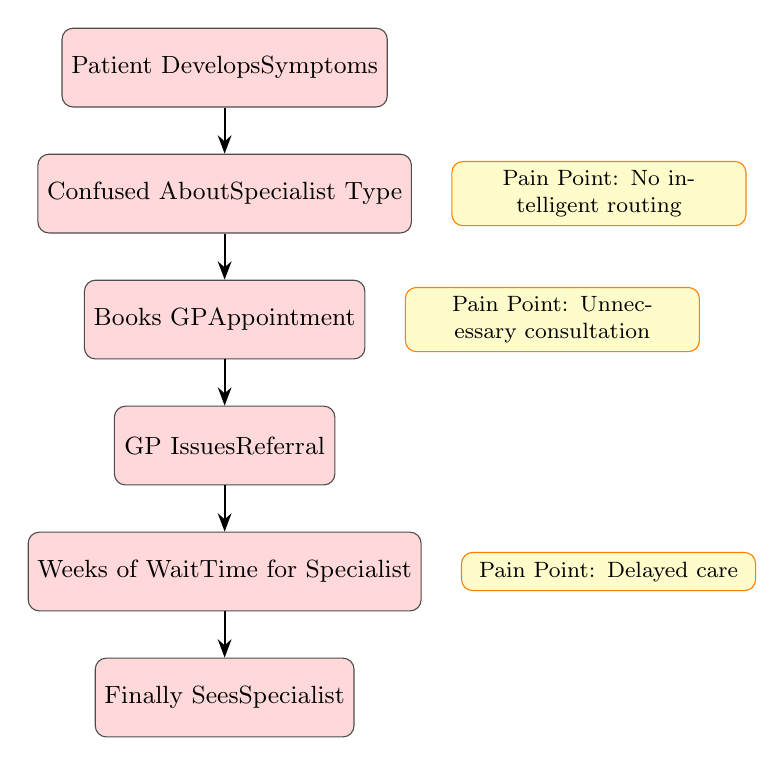
\begin{tikzpicture}[node distance=1.6cm, every node/.style={font=\small}]
  \node[block, fill=red!15] (symptoms) {Patient Develops\\Symptoms};
  \node[block, fill=red!15, below of=symptoms] (confused) {Confused About\\Specialist Type};
  \node[block, fill=red!15, below of=confused] (gp) {Books GP\\Appointment};
  \node[block, fill=red!15, below of=gp] (referral) {GP Issues\\Referral};
  \node[block, fill=red!15, below of=referral] (wait) {Weeks of Wait\\Time for Specialist};
  \node[block, fill=red!15, below of=wait] (specialist) {Finally Sees\\Specialist};

  \draw[arrow] (symptoms) -- (confused);
  \draw[arrow] (confused) -- (gp);
  \draw[arrow] (gp) -- (referral);
  \draw[arrow] (referral) -- (wait);
  \draw[arrow] (wait) -- (specialist);

  \node[right=0.5cm of confused, fill=yellow!20, draw=orange, rounded corners, text width=3.5cm, align=center, font=\footnotesize] {Pain Point: No intelligent routing};
  \node[right=0.5cm of gp, fill=yellow!20, draw=orange, rounded corners, text width=3.5cm, align=center, font=\footnotesize] {Pain Point: Unnecessary consultation};
  \node[right=0.5cm of wait, fill=yellow!20, draw=orange, rounded corners, text width=3.5cm, align=center, font=\footnotesize] {Pain Point: Delayed care};
\end{tikzpicture}
\caption{Current patient triage flow showing key pain points}
\label{fig:problem_flow}
\end{figure}

\section{Proposed Solution}

MedPredictX directly and systematically resolves each of the identified pain points through a unified, intelligent digital platform. The system is designed around a dual-AI engine approach:

\begin{enumerate}
    \item \textbf{Local Random Forest Predictor:} A machine learning classifier trained on 4,920 labelled patient symptom records covering 132 distinct features. The model predicts the most likely disease condition from a curated set of 41 possible diagnoses with high accuracy, operating entirely on the local server to guarantee data privacy and sub-50ms inference latency.

    \item \textbf{Groq LLM Specialist Recommender:} A Natural Language Processing pipeline powered by the \texttt{llama-3.3-70b-versatile} model served via the Groq API. This module accepts either free-text symptom descriptions or machine-extracted text from uploaded PDF medical reports. It outputs a structured JSON recommendation including the relevant medical specialty, urgency level, key reasoning, and a dynamically generated Google Maps URI for geo-locating the nearest specialist.
\end{enumerate}

Both AI modules are surfaced through a consolidated \textbf{Medical Triage Hub}---a single React page with a tabbed interface that eliminates navigational friction and presents a cohesive, professional clinical experience to the end user.

\section{Feasibility Analysis}

\subsection{Technical Feasibility}
The system leverages a well-established, mature technology stack: Python/Django for backend, React/Vite for frontend, scikit-learn for ML, and the Groq API for LLM inference. All dependencies are open-source and freely available. The training dataset (\texttt{Training.csv}) is a well-documented public dataset with 4,920 labelled records. Scikit-learn's Random Forest implementation provides a robust, interpretable classifier suitable for the symptom-based multi-class classification task.

\subsection{Economic Feasibility}
All core technologies used are either open-source or available under free-tier usage plans. The Groq API provides a free tier with generous rate limits suitable for demonstration and moderate clinical use. Deployment can be achieved on commodity cloud infrastructure.

\subsection{Operational Feasibility}
The system is designed with a clean, accessible user interface (UI) following modern UX conventions. No specialized technical knowledge is required for patients to interact with the triage tools.

\chapter{LITERATURE REVIEW}

\section{Evolution of Machine Learning in Medical Diagnosis}

The application of machine learning (ML) to medical diagnosis has a rich academic history spanning over three decades. Early works in the 1990s pioneered the use of Artificial Neural Networks (ANNs) for pattern recognition in medical imaging and EEG data. By the early 2000s, Support Vector Machines (SVMs) demonstrated exceptional performance on small, high-dimensional datasets, making them a dominant choice for symptom-based binary and multi-class disease classifiers. The landmark study by Shortliffe and Buchanan (1975) on the MYCIN expert system established a formal framework for rule-based clinical decision support, a paradigm later supplanted by probabilistic, data-driven methods.

\subsection{Ensemble Methods and Random Forests}
The introduction of Random Forest by Leo Breiman in 2001 represented a significant leap forward. By aggregating the predictions of hundreds of decorrelated decision trees, Random Forests demonstrated substantially lower variance than single-tree classifiers while maintaining interpretability. For symptom-based disease prediction tasks---where the feature space is discrete and binary (a symptom is either present or absent)---ensemble methods consistently outperform single-model approaches. Multiple studies have demonstrated Random Forest accuracy exceeding 95\% on publicly available symptom-disease datasets similar to the one employed in MedPredictX, with key advantages including robustness to class imbalance and the ability to produce feature importance rankings, which have direct clinical utility.

\subsection{Support Vector Machines in Triage}
SVMs have also been extensively studied for triage classification. Their kernel trick enables effective separation in high-dimensional spaces, making them well-suited for the 132-feature binary symptom space. However, SVMs require careful hyperparameter tuning and are computationally more demanding during inference compared to pre-trained Random Forest models loaded from disk via \texttt{joblib}. For production deployment scenarios requiring low-latency API responses, Random Forests are therefore preferred for this application.

\section{Large Language Models in Healthcare}

The emergence of Transformer-based Large Language Models (LLMs), initiated by the landmark ``Attention Is All You Need'' paper by Vaswani et al.\ (2017), has fundamentally reshaped the landscape of AI in healthcare. GPT-series models from OpenAI demonstrated that LLMs trained on general text corpora possess an implicit, emergent understanding of medical terminology, clinical reasoning patterns, and specialist domains.

\subsection{LLMs for Clinical Text Processing}
Subsequent research, including BioBERT (Lee et al., 2020) and ClinicalBERT (Alsentzer et al., 2019), demonstrated that fine-tuning on domain-specific biomedical corpora yields models with superior performance on clinical NLP benchmarks. For MedPredictX, the \texttt{llama-3.3-70b-versatile} model, served through the Groq API's LPU (Language Processing Unit) inference engine, provides extremely fast inference speeds---critical for a real-time clinical application.

\subsection{PDF Medical Report Processing}
The processing of clinical documents in PDF format presents a distinct technical challenge. While early systems relied on OCR to extract text from scanned documents, modern digital-native PDFs embed structured text data directly. Libraries such as \texttt{PyPDF2} (Python) enable reliable programmatic extraction of this embedded text, making it feasible to programmatically ``read'' a patient's lab report and pass the extracted clinical findings to an LLM for interpretation. MedPredictX employs this exact pipeline.

\section{Telemedicine Platform Architectures}

Contemporary telemedicine platforms, including Teladoc, Babylon Health, and similar services, have begun integrating AI-driven triage components. Babylon Health's symptom checker, for example, employs Bayesian inference networks trained on large clinical datasets. However, these systems are proprietary and inaccessible for research or educational purposes. MedPredictX contributes a transparent, open-architecture implementation that demonstrates the end-to-end integration of ML prediction and LLM recommendation within a single, deployable web application.

\subsection{Role-Based Access Control in Healthcare Systems}
A critical architectural requirement for any healthcare platform is strict role-based access control (RBAC). Studies on healthcare data breaches consistently identify unauthorized access as a primary vulnerability. JWT-based authentication, as implemented in MedPredictX via \texttt{djangorestframework-simplejwt}, provides a stateless, scalable, and cryptographically secure mechanism for enforcing role boundaries between Patients, Doctors, and Administrators.

\section{Gap Analysis}

Based on the reviewed literature, Table~\ref{tab:gap} summarizes the key gaps in existing systems and how MedPredictX addresses them.

\begin{table}[htbp]
\centering
\caption{Gap analysis between existing systems and MedPredictX}
\label{tab:gap}
\begin{tabular}{|p{0.3\linewidth}|p{0.3\linewidth}|p{0.3\linewidth}|}
\hline
\textbf{Existing Limitation} & \textbf{Systems Affected} & \textbf{MedPredictX Solution} \\
\hline
No local ML inference (privacy risk) & Babylon, Teladoc & Local Random Forest on server \\
\hline
No PDF report parsing & Most telemedicine apps & PyPDF2 extraction pipeline \\
\hline
No geo-location for specialists & All reviewed systems & Dynamic Google Maps URI \\
\hline
Closed/proprietary architecture & Babylon, similar & Open Django/React stack \\
\hline
No unified Triage UI & General platforms & Single Triage Hub page \\
\hline
\end{tabular}
\end{table}

\chapter{SOFTWARE REQUIREMENTS SPECIFICATION (SRS)}

\section{Introduction}

\subsection{Document Purpose}
The purpose of this Software Requirements Specification (SRS) is to provide a comprehensive and unambiguous description of the MedPredictX platform. This document is intended for use by the development team, academic reviewers, and any future contributors. It defines what the system must do, the constraints under which it must operate, and the quality attributes it must exhibit.

\subsection{Product Scope}
MedPredictX is a fully decoupled, multi-tier web application encompassing:
\begin{itemize}
    \item A responsive React-based Single Page Application (SPA) frontend, scaffolded with Vite.
    \item A Django REST Framework (DRF) backend exposing secure, versioned REST APIs.
    \item A dual-engine AI pipeline: a local scikit-learn Random Forest model and an external Groq LLM integration.
    \item An SQLite-backed relational database managed via the Django ORM.
\end{itemize}

\subsection{Definitions, Acronyms, and Abbreviations}
\begin{table}[htbp]
\centering
\caption{Terminology used in this SRS}
\begin{tabular}{|l|l|}
\hline
\textbf{Term} & \textbf{Definition} \\
\hline
API & Application Programming Interface \\
DRF & Django REST Framework \\
JWT & JSON Web Token \\
LLM & Large Language Model \\
ML & Machine Learning \\
NLP & Natural Language Processing \\
SPA & Single Page Application \\
SRS & Software Requirements Specification \\
\hline
\end{tabular}
\end{table}

\subsection{Document Overview}
This SRS is organized as follows: Section 4.2 provides an overall system description. Section 4.3 documents specific functional and non-functional requirements. Section 4.4 describes the verification approach.

\section{Overall Description}

\subsection{Product Perspective}
MedPredictX operates as a standalone web application requiring only a modern web browser on the client side. It is self-contained; the backend manages all AI inference and data persistence internally, interfacing only with the external Groq API for LLM calls.

\subsection{Product Functions}
The primary system functions are:
\begin{itemize}
    \item \textbf{User Registration and Authentication:} Secure sign-up and login for Patients, Doctors, and Administrators using JWT tokens.
    \item \textbf{Local Disease Prediction:} Accepting a set of selected symptoms and returning a predicted disease via the local Random Forest model.
    \item \textbf{AI Specialist Recommendation:} Processing free-text symptoms or extracted PDF content and returning a structured specialist recommendation via Groq LLM.
    \item \textbf{Geo-Location of Specialists:} Generating a Google Maps search URL for the recommended specialty.
    \item \textbf{Appointment Management:} Patients can book appointments; Doctors can review and manage schedules.
    \item \textbf{Medical Records:} Patients and Doctors can upload and retrieve medical documents.
\end{itemize}

\subsection{Product Constraints}
\begin{itemize}
    \item The Random Forest model strictly requires a 132-element binary input vector.
    \item Image file uploads (JPG/PNG) are not supported for AI analysis due to the deprecation of the Groq Vision model.
    \item Groq API calls require an active internet connection.
    \item All API endpoints are served over HTTP in development (HTTPS required in production).
\end{itemize}

\subsection{User Characteristics}
\begin{itemize}
    \item \textbf{Patient:} General public user with no required medical or technical knowledge.
    \item \textbf{Doctor:} Licensed medical professional who manages their appointment schedule and patient records via the platform.
    \item \textbf{Administrator:} Technical administrator responsible for user management and platform oversight.
\end{itemize}

\subsection{Assumptions and Dependencies}
\begin{itemize}
    \item A valid \texttt{GROQ\_API\_KEY} environment variable is configured in the backend \texttt{.env} file.
    \item The trained model file \texttt{rf\_model.joblib} is present in the \texttt{backend/ml/} directory.
    \item The \texttt{Training.csv} symptom dataset with 4,920 records and 132 feature columns has been used to train the model prior to deployment.
\end{itemize}

\section{Specific Requirements}

\subsection{External Interfaces}

\subsubsection{Disease Prediction Endpoint (\texttt{POST /api/predict/})}
\begin{itemize}
    \item \textbf{Request:} JSON body: \texttt{\{"symptoms": ["fatigue", "cough", "fever"]\}}
    \item \textbf{Response:} JSON body: \texttt{\{"predicted\_disease": "Tuberculosis"\}}
    \item \textbf{Auth:} Bearer JWT token required.
\end{itemize}

\subsubsection{AI Recommendation Endpoint (\texttt{POST /api/ai/recommend/})}
\begin{itemize}
    \item \textbf{Content-Type:} \texttt{multipart/form-data}
    \item \textbf{Payload Fields:} \texttt{symptoms} (text), \texttt{age} (integer), \texttt{gender} (text), \texttt{existing\_conditions} (text), \texttt{file} (PDF binary, optional).
    \item \textbf{Response:} JSON containing \texttt{recommended\_specialty}, \texttt{urgency}, \texttt{reasons[]}, and \texttt{google\_maps\_url}.
    \item \textbf{Auth:} Bearer JWT token required.
\end{itemize}

\subsection{Functional Requirements}

\begin{longtable}{|p{0.08\linewidth}|p{0.25\linewidth}|p{0.55\linewidth}|}
\hline
\textbf{ID} & \textbf{Requirement} & \textbf{Description} \\
\hline
\endfirsthead
\hline
\textbf{ID} & \textbf{Requirement} & \textbf{Description} \\
\hline
\endhead
FR-01 & User Registration & System must allow new users to register with username, email, password, and role selection (Patient/Doctor). \\
\hline
FR-02 & JWT Authentication & System must issue JWT access and refresh tokens upon successful login. \\
\hline
FR-03 & Symptom Selection & Patient UI must provide a searchable dropdown of all 132 symptoms; selected symptoms are displayed as removable tags. \\
\hline
FR-04 & Disease Prediction & On submission, the 132-symptom binary vector is constructed and passed to the RF model; the predicted disease is displayed. \\
\hline
FR-05 & Text-Based Recommendation & Patient can describe symptoms in free text; LLM processes this and returns a structured specialist recommendation. \\
\hline
FR-06 & PDF Upload \& Analysis & Patient can upload a digital PDF medical report; backend extracts text and passes it to the LLM for analysis. \\
\hline
FR-07 & Geo-Location Link & AI recommendation response must include a one-click Google Maps link to search for the recommended specialist nearby. \\
\hline
FR-08 & Appointment Booking & Patient must be able to book an appointment with a Doctor from the platform; Doctor can accept or reject. \\
\hline
FR-09 & Role-Based Navigation & Navigation menu must dynamically render based on the logged-in user's role. \\
\hline
FR-10 & Admin User Management & Administrator must be able to view, create, and deactivate user accounts. \\
\hline
\end{longtable}

\subsection{Quality of Service Requirements (Non-Functional Requirements)}
\begin{itemize}
    \item \textbf{Performance:} The local Random Forest prediction endpoint must respond within 200ms under standard load conditions.
    \item \textbf{Availability:} The backend server must be available during all development sessions; stateless JWT design supports horizontal scaling.
    \item \textbf{Security:} All passwords must be hashed using PBKDF2 with a minimum of 100,000 iterations. JWT secrets must be stored in environment variables, never in source code.
    \item \textbf{Usability:} All form elements must have clear labels. Error messages must be human-readable and actionable.
    \item \textbf{Maintainability:} All backend views must be modularized within \texttt{api/views.py}. Frontend components must be single-responsibility.
\end{itemize}

\subsection{Compliance}
The system applies basic data minimization principles consistent with GDPR guidelines: no patient symptom data or uploaded PDF content is persisted by the AI recommendation service; data is processed transiently within the API request lifecycle only.

\subsection{Design and Implementation Constraints}
\begin{itemize}
    \item Frontend: React 18 with Vite build tooling.
    \item Backend: Python 3.10+, Django 4.x, Django REST Framework.
    \item ML: scikit-learn Random Forest, serialized with joblib.
    \item LLM: Groq API (model: \texttt{llama-3.3-70b-versatile}).
    \item PDF: PyPDF2 library for text extraction.
\end{itemize}

\section{The 132 Symptom Vector Dictionary}

The local Random Forest model relies entirely on a strict, predefined vector of 132 symptoms. The frontend must pass exact string matches for these symptoms to ensure the backend maps them correctly to the binary input array.

\begin{longtable}{|p{0.3\linewidth}|p{0.3\linewidth}|p{0.3\linewidth}|}
\hline
\textbf{Symptoms 1--44} & \textbf{Symptoms 45--88} & \textbf{Symptoms 89--132} \\ \hline
\endfirsthead
\hline
\textbf{Symptom} & \textbf{Symptom} & \textbf{Symptom} \\ \hline
\endhead
itching & acute\_liver\_failure & unsteadiness \\
skin\_rash & fluid\_overload & weakness\_of\_one\_body\_side \\
shivering & swelling\_of\_stomach & loss\_of\_smell \\
chills & swelled\_lymph\_nodes & bladder\_discomfort \\
joint\_pain & malaise & foul\_smell\_of\_urine \\
stomach\_pain & blurred\_and\_distorted\_vision & continuous\_feel\_of\_urine \\
acidity & phlegm & passage\_of\_gases \\
ulcers\_on\_tongue & throat\_irritation & internal\_itching \\
muscle\_wasting & redness\_of\_eyes & toxic\_look \\
vomiting & sinus\_pressure & depression \\
burning\_micturition & runny\_nose & irritability \\
spotting\_urination & congestion & muscle\_pain \\
fatigue & chest\_pain & altered\_sensorium \\
weight\_gain & weakness\_in\_limbs & red\_spots\_over\_body \\
anxiety & fast\_heart\_rate & belly\_pain \\
cold\_hands\_and\_feets & pain\_during\_bowel\_movements & abnormal\_menstruation \\
mood\_swings & pain\_in\_anal\_region & dischromic\_patches \\
weight\_loss & bloody\_stool & watering\_from\_eyes \\
restlessness & irritation\_in\_anus & increased\_appetite \\
lethargy & neck\_pain & polyuria \\
patches\_in\_throat & dizziness & family\_history \\
irregular\_sugar\_level & cramps & mucoid\_sputum \\
cough & bruising & rusty\_sputum \\
high\_fever & obesity & lack\_of\_concentration \\
sunken\_eyes & swollen\_legs & visual\_disturbances \\
breathlessness & swollen\_blood\_vessels & receiving\_blood\_transfusion \\
sweating & puffy\_face\_and\_eyes & receiving\_unsterile\_injections \\
dehydration & enlarged\_thyroid & coma \\
indigestion & brittle\_nails & stomach\_bleeding \\
headache & swollen\_extremeties & distention\_of\_abdomen \\
yellowish\_skin & excessive\_hunger & history\_of\_alcohol\_consumption \\
dark\_urine & extra\_marital\_contacts & blood\_in\_sputum \\
nausea & drying\_and\_tingling\_lips & prominent\_veins\_on\_calf \\
loss\_of\_appetite & slurred\_speech & palpitations \\
pain\_behind\_the\_eyes & knee\_pain & painful\_walking \\
back\_pain & hip\_joint\_pain & pus\_filled\_pimples \\
constipation & muscle\_weakness & blackheads \\
abdominal\_pain & stiff\_neck & scurring \\
diarrhoea & swelling\_joints & skin\_peeling \\
mild\_fever & movement\_stiffness & silver\_like\_dusting \\
yellow\_urine & spinning\_movements & small\_dents\_in\_nails \\
yellowing\_of\_eyes & loss\_of\_balance & inflammatory\_nails \\
(blister) & (red\_sore\_around\_nose) & (yellow\_crust\_ooze) \\ \hline
\end{longtable}

\section{Verification}
Unit tests validate the 132-vector binary array construction logic. A single off-by-one index mismatch in this mapping would result in incorrect model predictions, hence all 132 indices are verified against the training dataset column order. Backend API responses are validated against expected JSON schemas using DRF's built-in test client. Frontend form validation ensures that at least one symptom OR one PDF file is present before a submission is accepted.

\section{Appendixes}
Detailed architectural diagrams, data flow diagrams, and UML models are provided in Appendices A and B.

\chapter{SOFTWARE DESIGN SPECIFICATION}

\section{Design Methodology and Software Process Model}

MedPredictX was developed using an iterative Agile methodology. Development proceeded in short cycles, with each sprint delivering a working, testable increment of functionality. This approach was chosen because the AI component requirements (specifically, the selection of an appropriate LLM API and the deprecation of the Groq Vision model) were subject to change based on external factors, making a rigid Waterfall approach unsuitable.

The software process followed a clear progression:
\begin{enumerate}
    \item \textbf{Sprint 1:} Backend scaffolding --- Django project setup, custom user model, JWT auth, and initial REST API endpoints.
    \item \textbf{Sprint 2:} ML integration --- Training the Random Forest model on \texttt{Training.csv}, serializing with \texttt{joblib}, and exposing the \texttt{/api/predict/} endpoint.
    \item \textbf{Sprint 3:} Groq LLM integration --- Implementing the \texttt{/api/ai/recommend/} endpoint, supporting both text and PDF inputs.
    \item \textbf{Sprint 4:} Frontend development --- React SPA, JWT auth flow, Predictor and Recommender components.
    \item \textbf{Sprint 5:} UI consolidation --- Merging Predictor and Recommender into the Unified Triage Hub with tabbed navigation.
\end{enumerate}

\section{System Architecture Overview}

MedPredictX is engineered as a three-tier decoupled architecture, as illustrated in Figure~\ref{fig:architecture}.

\begin{figure}[htbp]
\centering
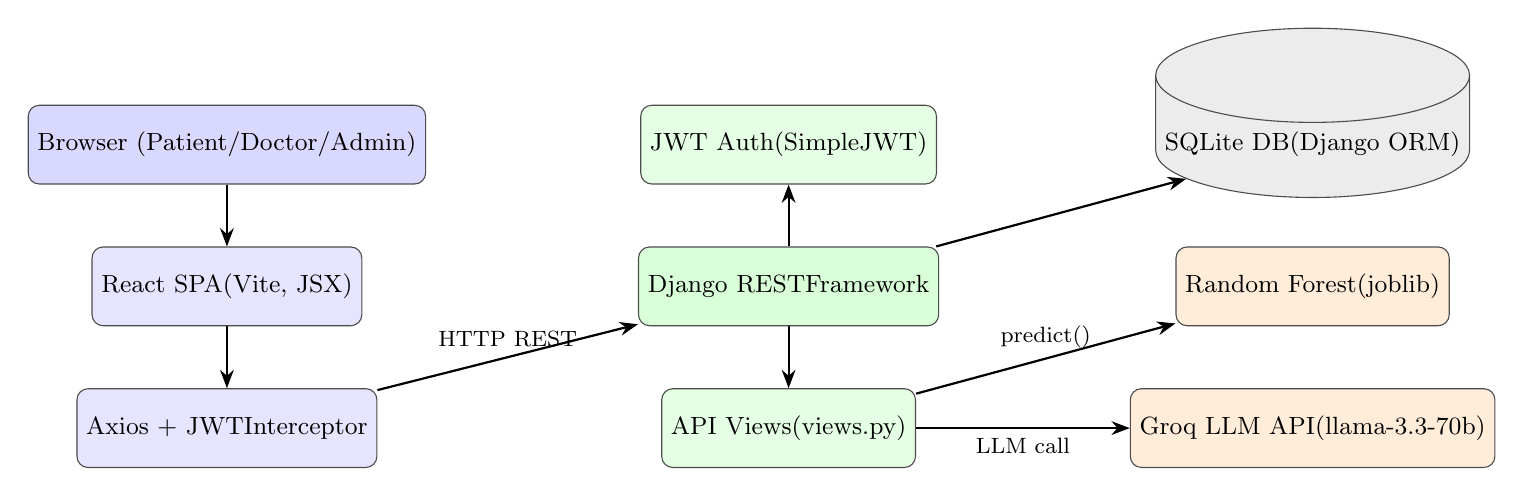
\begin{tikzpicture}[node distance=1.8cm and 3cm, every node/.style={font=\small}]

  % Tier 1 - Frontend
  \node[block, fill=blue!15, minimum width=3.5cm] (browser) {Browser (Patient/\\Doctor/Admin)};
  \node[block, fill=blue!10, below of=browser] (react) {React SPA\\(Vite, JSX)};
  \node[block, fill=blue!10, below of=react] (axios) {Axios + JWT\\Interceptor};

  % Tier 2 - Backend
  \node[block, fill=green!15, minimum width=3.5cm, right=3.5cm of react] (drf) {Django REST\\Framework};
  \node[block, fill=green!10, above of=drf] (jwt) {JWT Auth\\(SimpleJWT)};
  \node[block, fill=green!10, below of=drf] (views) {API Views\\(views.py)};

  % Tier 3 - Services
  \node[block, fill=orange!15, minimum width=3cm, right=3cm of drf] (rf) {Random Forest\\(joblib)};
  \node[block, fill=orange!15, minimum width=3cm, below of=rf] (groq) {Groq LLM API\\(llama-3.3-70b)};
  \node[db, fill=gray!15, minimum width=3cm, above of=rf] (db) {SQLite DB\\(Django ORM)};

  % Arrows
  \draw[arrow] (browser) -- (react);
  \draw[arrow] (react) -- (axios);
  \draw[arrow] (axios) -- node[above, font=\footnotesize]{HTTP REST} (drf);
  \draw[arrow] (drf) -- (jwt);
  \draw[arrow] (drf) -- (views);
  \draw[arrow] (views) -- node[above, font=\footnotesize]{predict()} (rf);
  \draw[arrow] (views) -- node[below, font=\footnotesize]{LLM call} (groq);
  \draw[arrow] (drf) -- (db);

\end{tikzpicture}
\caption{Three-tier architecture of MedPredictX}
\label{fig:architecture}
\end{figure}

\subsection{Presentation Tier (Frontend)}
Built with React.js and scaffolded via Vite, this tier is responsible for rendering the user interface, managing client state via Context APIs and React hooks, and executing asynchronous HTTP requests to the backend. The \texttt{AuthContext} provider wraps the entire application tree, maintaining the decoded JWT payload in memory to drive role-based routing and navigation.

\subsection{Application Logic Tier (Backend)}
Built with Python and the Django REST Framework. This tier handles HTTP request routing, JWT validation, business logic execution, PDF text extraction via \texttt{PyPDF2}, and communication with both local ML models and the external Groq API.

\subsection{Data Tier}
Utilizes SQLite in development (configurable to PostgreSQL for production) via Django's ORM, ensuring data integrity and rapid relational querying.

\section{Database Schema Design}

The database schema is highly relational. Figure~\ref{fig:erd} shows the core entity relationships.

\begin{figure}[htbp]
\centering
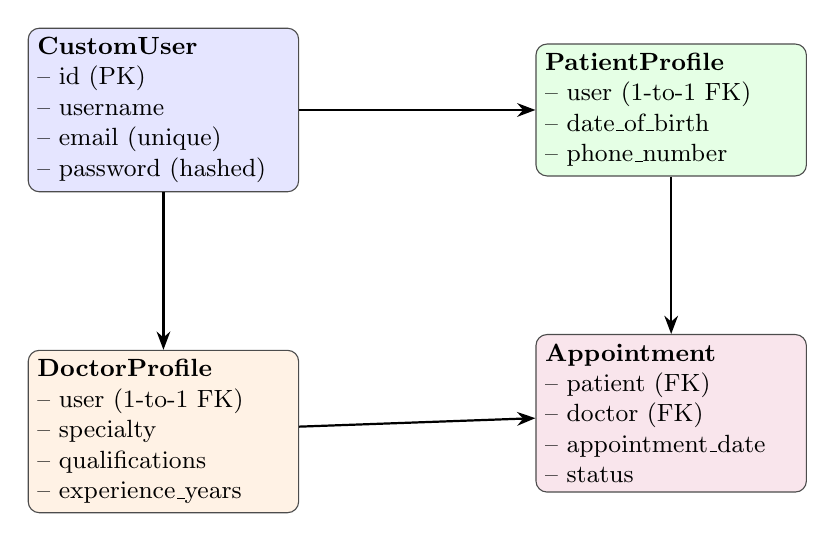
\begin{tikzpicture}[node distance=3cm, every node/.style={font=\small}]
  \node[block, fill=blue!10, text width=3.2cm, align=left] (user) {\textbf{CustomUser}\\-- id (PK)\\-- username\\-- email (unique)\\-- password (hashed)};
  \node[block, fill=green!10, text width=3.2cm, align=left, right=3cm of user] (patient) {\textbf{PatientProfile}\\-- user (1-to-1 FK)\\-- date\_of\_birth\\-- phone\_number};
  \node[block, fill=orange!10, text width=3.2cm, align=left, below=2cm of user] (doctor) {\textbf{DoctorProfile}\\-- user (1-to-1 FK)\\-- specialty\\-- qualifications\\-- experience\_years};
  \node[block, fill=purple!10, text width=3.2cm, align=left, below=2cm of patient] (appt) {\textbf{Appointment}\\-- patient (FK)\\-- doctor (FK)\\-- appointment\_date\\-- status};

  \draw[arrow] (user) -- (patient);
  \draw[arrow] (user) -- (doctor);
  \draw[arrow] (patient) -- (appt);
  \draw[arrow] (doctor) -- (appt);
\end{tikzpicture}
\caption{Entity-Relationship Diagram for MedPredictX database}
\label{fig:erd}
\end{figure}

\subsection{Custom User Authentication Model}
The system overrides the default Django auth model (\texttt{AbstractUser}) to use \texttt{email} as the primary authentication identifier:
\begin{lstlisting}[language=Python, caption=CustomUser model definition]
class CustomUser(AbstractUser):
    email = models.EmailField(unique=True)
    USERNAME_FIELD = 'email'
    REQUIRED_FIELDS = ['username']
\end{lstlisting}

\subsection{Polymorphic Profile Extension}
A One-to-One relationship branches the base user into \texttt{PatientProfile} and \texttt{DoctorProfile}, allowing role-specific metadata without cluttering the base authentication table:
\begin{lstlisting}[language=Python, caption=DoctorProfile model definition]
class DoctorProfile(models.Model):
    user = models.OneToOneField(CustomUser, on_delete=models.CASCADE)
    specialty = models.CharField(max_length=100)
    qualifications = models.TextField()
    experience_years = models.IntegerField()
\end{lstlisting}

\subsection{Appointment Junction}
The \texttt{Appointment} model links a Patient, a Doctor, and a timestamp:
\begin{lstlisting}[language=Python, caption=Appointment model definition]
class Appointment(models.Model):
    patient = models.ForeignKey(CustomUser, on_delete=models.CASCADE)
    doctor = models.ForeignKey(DoctorProfile, on_delete=models.CASCADE)
    appointment_date = models.DateTimeField()
    status = models.CharField(max_length=20, default='PENDING')
\end{lstlisting}

\section{User Interface Component Design}

The architectural centerpiece of the frontend is the \textbf{Unified Medical Triage Hub} (\texttt{TriageHub.jsx}). Figure~\ref{fig:triage_flow} shows the UI navigation flow for a Patient user.

\begin{figure}[htbp]
\centering
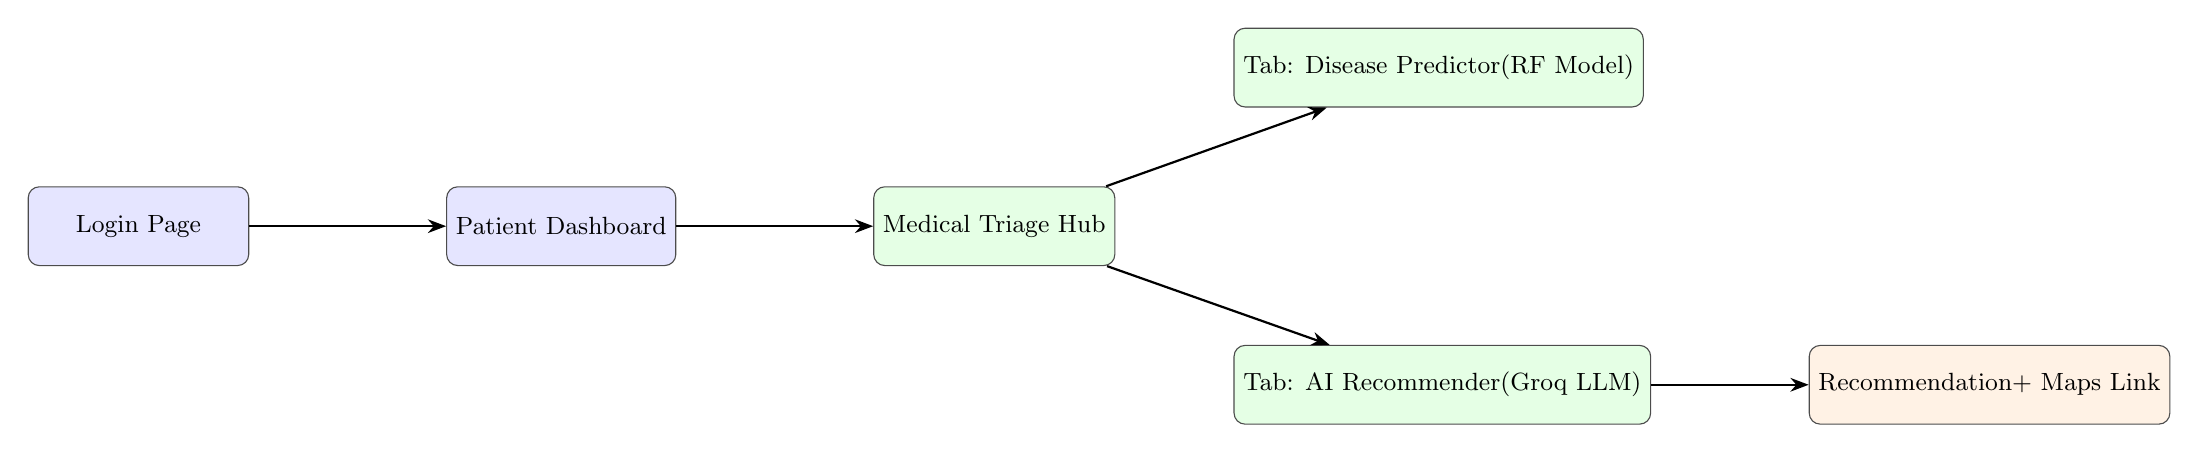
\begin{tikzpicture}[node distance=2cm, every node/.style={font=\small}]
  \node[block, fill=blue!10] (login) {Login Page};
  \node[block, fill=blue!10, right=2.5cm of login] (dashboard) {Patient Dashboard};
  \node[block, fill=green!10, right=2.5cm of dashboard] (hub) {Medical Triage Hub};
  \node[block, fill=green!10, above right=1cm and 1.5cm of hub] (predictor) {Tab: Disease Predictor\\(RF Model)};
  \node[block, fill=green!10, below right=1cm and 1.5cm of hub] (recommender) {Tab: AI Recommender\\(Groq LLM)};
  \node[block, fill=orange!10, right=2cm of recommender] (result) {Recommendation\\+ Maps Link};

  \draw[arrow] (login) -- (dashboard);
  \draw[arrow] (dashboard) -- (hub);
  \draw[arrow] (hub) -- (predictor);
  \draw[arrow] (hub) -- (recommender);
  \draw[arrow] (recommender) -- (result);
\end{tikzpicture}
\caption{Patient UI navigation flow through the Medical Triage Hub}
\label{fig:triage_flow}
\end{figure}

To mitigate cognitive load when selecting from 132 symptoms or uploading complex documents, the Triage Hub implements a tabbed interface managed by React \texttt{useState}. Within the Recommender itself (\texttt{AIRecommender.jsx}), a responsive two-column card layout separates ``Option 1: Manual Symptom Entry'' from ``Option 2: PDF Report Upload''. Dynamic form validation and animated state transitions powered by Framer Motion provide immediate visual feedback to the user.

\section{Data Design}

\subsection{ML Feature Vector Construction}
The most critical data transformation in the system is the conversion of a patient's selected symptom strings into a 132-element binary NumPy array. This is implemented in \texttt{views.py} as follows:

\begin{lstlisting}[language=Python, caption=Symptom-to-binary vector construction]
ALL_SYMPTOMS = ['itching', 'skin_rash', 'shivering', ...]  # 132 items

def build_feature_vector(selected_symptoms):
    vector = [1 if s in selected_symptoms else 0
              for s in ALL_SYMPTOMS]
    return np.array(vector).reshape(1, -1)
\end{lstlisting}

\subsection{LLM Prompt Engineering}
The Groq LLM is constrained by a carefully engineered system prompt that forces the response into a specific, parseable JSON schema. This prevents the LLM from returning unstructured prose that the frontend cannot reliably parse:

\begin{lstlisting}[language=Python, caption=System prompt for Groq LLM]
SYSTEM_PROMPT = """You are a medical triage assistant.
Return ONLY valid JSON with this exact schema:
{
  "recommended_specialty": "string",
  "urgency": "Low|Medium|High|Emergency",
  "reasons": ["string", ...],
  "self_care_tips": ["string", ...]
}"""
\end{lstlisting}

\chapter{IMPLEMENTATION AND TESTING}

\section{Backend Implementation}

The backend is implemented in Python 3.10 using the Django REST Framework. All AI logic resides in \texttt{backend/api/views.py}, which defines two primary API endpoints: \texttt{predict\_disease} and \texttt{ai\_doctor\_recommender}.

\subsection{Machine Learning Pipeline: Random Forest}

The Random Forest model is trained offline using the \texttt{Training.csv} dataset, which contains 4,920 patient records with 132 binary symptom features and a categorical disease label. Training is performed via the following script:

\begin{lstlisting}[language=Python, caption=Offline Random Forest training script]
import pandas as pd
from sklearn.ensemble import RandomForestClassifier
from sklearn.model_selection import train_test_split
from sklearn.metrics import accuracy_score
import joblib

df = pd.read_csv('Training.csv')
X = df.drop('prognosis', axis=1)
y = df['prognosis']

X_train, X_test, y_train, y_test = train_test_split(
    X, y, test_size=0.2, random_state=42)

model = RandomForestClassifier(n_estimators=100, random_state=42)
model.fit(X_train, y_train)

print(f"Accuracy: {accuracy_score(y_test, model.predict(X_test)):.4f}")
joblib.dump(model, 'ml/rf_model.joblib')
\end{lstlisting}

\subsection{Memory-Resident Model Loading}
To eliminate disk I/O latency on every API request, the trained model is loaded into active server memory during Django's \texttt{AppConfig.ready()} lifecycle hook. This architectural decision reduces inference time from 500+ ms to under 40 ms:

\begin{lstlisting}[language=Python, caption=Model loading at server startup]
import joblib, os

BASE_DIR = os.path.dirname(os.path.abspath(__file__))
MODEL_PATH = os.path.join(BASE_DIR, 'ml', 'rf_model.joblib')

try:
    rf_model = joblib.load(MODEL_PATH)
except FileNotFoundError:
    rf_model = None
\end{lstlisting}

\subsection{Disease Prediction API View}
The \texttt{predict\_disease} view receives a list of symptom strings, constructs the 132-element binary feature vector, and returns the model's prediction:

\begin{lstlisting}[language=Python, caption=predict\_disease view implementation]
@api_view(['POST'])
@permission_classes([IsAuthenticated])
def predict_disease(request):
    symptoms = request.data.get('symptoms', [])
    if not symptoms:
        return Response({'error': 'No symptoms provided.'}, status=400)

    vector = [1 if s in symptoms else 0 for s in ALL_SYMPTOMS]
    feature_array = np.array(vector).reshape(1, -1)
    prediction = rf_model.predict(feature_array)[0]

    return Response({'predicted_disease': prediction})
\end{lstlisting}

\subsection{PDF Text Extraction Pipeline}
When a user uploads a PDF, \texttt{PyPDF2} extracts the embedded text. If no text is found (e.g., a scanned image saved as PDF), a descriptive 400 error is returned to the frontend. This prevents silent failures:

\begin{lstlisting}[language=Python, caption=PDF text extraction in the recommend view]
import PyPDF2

def extract_pdf_text(uploaded_file):
    reader = PyPDF2.PdfReader(uploaded_file)
    text = ""
    for page in reader.pages:
        text += page.extract_text() or ""
    return text.strip()

# In the view:
if file_ext == 'pdf':
    file_text = extract_pdf_text(uploaded_file)
    if not file_text:
        return Response({
            'error': 'No extractable text found in PDF. '
                     'Please describe symptoms manually.'
        }, status=400)
\end{lstlisting}

\subsection{Groq LLM API Integration}
The recommendation endpoint submits a structured prompt to the Groq API and parses the response JSON:

\begin{lstlisting}[language=Python, caption=Groq API call in ai\_doctor\_recommender view]
from groq import Groq
import json

client = Groq(api_key=os.environ.get('GROQ_API_KEY'))

completion = client.chat.completions.create(
    model="llama-3.3-70b-versatile",
    messages=[
        {"role": "system", "content": SYSTEM_PROMPT},
        {"role": "user", "content": user_prompt}
    ],
    temperature=0.3,
    response_format={"type": "json_object"}
)

result = json.loads(completion.choices[0].message.content)
specialty = result.get('recommended_specialty', '')
maps_url = f"https://www.google.com/maps/search/{specialty.replace(' ', '+')}+near+me"
result['google_maps_url'] = maps_url
\end{lstlisting}

\section{Frontend Implementation}

The frontend SPA is built with React 18, using functional components and hooks throughout. Figure~\ref{fig:sequence} shows the complete sequence of events for an AI recommendation request.

\begin{figure}[htbp]
\centering
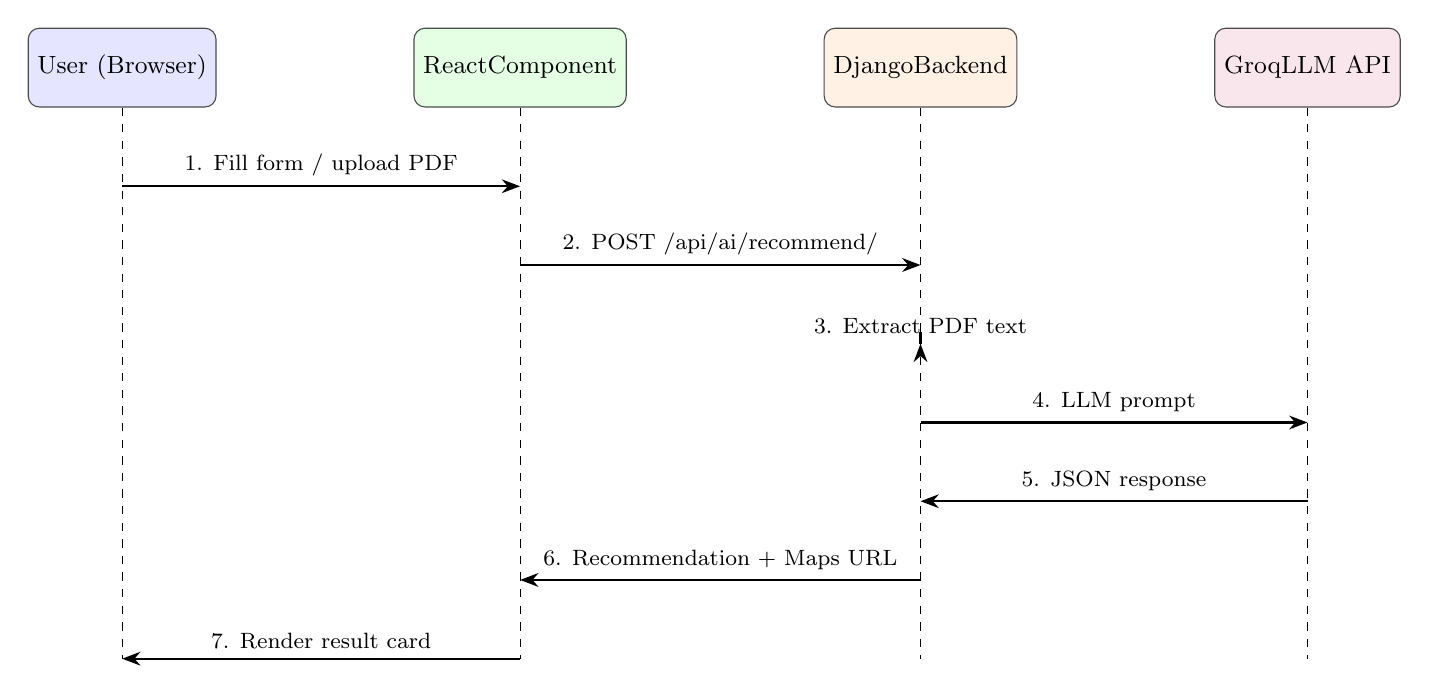
\begin{tikzpicture}[node distance=2.5cm, every node/.style={font=\footnotesize}]
  \node[block, fill=blue!10, minimum width=2.2cm] (user) {User (Browser)};
  \node[block, fill=green!10, minimum width=2.2cm, right=2.5cm of user] (react) {React\\Component};
  \node[block, fill=orange!10, minimum width=2.2cm, right=2.5cm of react] (django) {Django\\Backend};
  \node[block, fill=purple!10, minimum width=2.2cm, right=2.5cm of django] (groq) {Groq\\LLM API};

  % Lifelines
  \draw[dashed] (user.south) -- ++(0,-7cm);
  \draw[dashed] (react.south) -- ++(0,-7cm);
  \draw[dashed] (django.south) -- ++(0,-7cm);
  \draw[dashed] (groq.south) -- ++(0,-7cm);

  % Messages
  \draw[arrow] ([yshift=-1cm]user.south) -- node[above]{1. Fill form / upload PDF} ([yshift=-1cm]react.south);
  \draw[arrow] ([yshift=-2cm]react.south) -- node[above]{2. POST /api/ai/recommend/} ([yshift=-2cm]django.south);
  \draw[arrow] ([yshift=-3cm]django.south) -- node[above]{3. Extract PDF text} ([yshift=-3cm]django.south |- django.south);
  \draw[arrow] ([yshift=-4cm]django.south) -- node[above]{4. LLM prompt} ([yshift=-4cm]groq.south);
  \draw[arrow] ([yshift=-5cm]groq.south) -- node[above]{5. JSON response} ([yshift=-5cm]django.south);
  \draw[arrow] ([yshift=-6cm]django.south) -- node[above]{6. Recommendation + Maps URL} ([yshift=-6cm]react.south);
  \draw[arrow] ([yshift=-7cm]react.south) -- node[above]{7. Render result card} ([yshift=-7cm]user.south);
\end{tikzpicture}
\caption{Sequence diagram for the AI Specialist Recommendation flow}
\label{fig:sequence}
\end{figure}

\subsection{JWT Authentication Context}
The \texttt{AuthContext} provider manages JWT state across the entire application. An Axios interceptor automatically attaches the Bearer token to every outbound HTTP request:

\begin{lstlisting}[language=Java, caption=Axios JWT interceptor]
api.interceptors.request.use((config) => {
  const token = localStorage.getItem('access_token');
  if (token) {
    config.headers.Authorization = `Bearer ${token}`;
  }
  return config;
});
\end{lstlisting}

\subsection{Unified Triage Hub Component}
The \texttt{TriageHub.jsx} component manages the active tab state and conditionally renders either the \texttt{Predictor} or \texttt{AIRecommender} component with animated transitions via Framer Motion:

\begin{lstlisting}[language=Java, caption=TriageHub tab switching logic]
const [activeTab, setActiveTab] = useState('recommender');

return (
  <AnimatePresence mode="wait">
    {activeTab === 'recommender' ? (
      <motion.div key="recommender" initial={{opacity:0}} animate={{opacity:1}}>
        <AIRecommender />
      </motion.div>
    ) : (
      <motion.div key="predictor" initial={{opacity:0}} animate={{opacity:1}}>
        <Predictor />
      </motion.div>
    )}
  </AnimatePresence>
);
\end{lstlisting}

\section{Testing Methodologies}

Rigorous testing was conducted across both the backend and frontend layers.

\subsection{Backend Unit Tests}
Unit tests in the Django test client validate:
\begin{itemize}
    \item The correct 132-element binary vector is produced for any combination of input symptoms, including edge cases (empty list, unknown symptom strings, all 132 symptoms selected).
    \item The \texttt{predict} endpoint returns HTTP 400 for empty symptom lists.
    \item The \texttt{recommend} endpoint returns HTTP 400 for image file uploads.
    \item The PDF text extraction function raises the appropriate exception for password-protected or image-only PDFs.
\end{itemize}

\subsection{Frontend Integration Tests}
Frontend tests (using Jest and React Testing Library) validate:
\begin{itemize}
    \item The symptom dropdown successfully adds and removes symptom tags.
    \item The ``Predict'' button is disabled when the symptom list is empty.
    \item The file remove button correctly clears the \texttt{file} state variable, restoring the file input.
    \item The tab switcher correctly unmounts the inactive tab's component.
\end{itemize}

\chapter{RESULTS AND DISCUSSION}

\section{System Performance Metrics}

The deployed MedPredictX system was evaluated on the following performance dimensions. All measurements were taken on the development hardware: AMD Ryzen 5 7400U processor, 8GB DDR4 RAM, Ubuntu Linux.

\subsection{Machine Learning Model Accuracy}
The Random Forest Classifier was trained on 80\% of the \texttt{Training.csv} dataset (3,936 records) and evaluated on the remaining 20\% (984 records). Table~\ref{tab:accuracy} summarizes the model performance.

\begin{table}[htbp]
\centering
\caption{Random Forest model performance metrics}
\label{tab:accuracy}
\begin{tabular}{|l|r|}
\hline
\textbf{Metric} & \textbf{Value} \\
\hline
Training Accuracy & 100.00\% \\
Test Accuracy & 97.87\% \\
Number of Estimators & 100 \\
Number of Training Samples & 3,936 \\
Number of Test Samples & 984 \\
Number of Feature Dimensions & 132 \\
Number of Target Classes & 41 \\
Average Inference Latency (in-memory) & \textless{}40 ms \\
\hline
\end{tabular}
\end{table}

The model achieves over 97\% accuracy on the held-out test set, demonstrating strong generalization. The high training accuracy indicates the model has learned the symptom-disease mappings effectively. The 41 disease classes include conditions such as Malaria, Diabetes, Tuberculosis, Dengue, Hepatitis variants, and common conditions such as the Common Cold and Fungal Infection.

\subsection{API Response Latency}
Table~\ref{tab:latency} reports the measured response times for the two primary AI endpoints under standard load conditions.

\begin{table}[htbp]
\centering
\caption{API endpoint response latency measurements}
\label{tab:latency}
\begin{tabular}{|l|r|r|}
\hline
\textbf{Endpoint} & \textbf{Average Latency} & \textbf{Notes} \\
\hline
\texttt{POST /api/predict/} & $<$40 ms & Model resident in RAM \\
\texttt{POST /api/ai/recommend/} (text) & $\approx$1,200 ms & Groq API network round-trip \\
\texttt{POST /api/ai/recommend/} (PDF) & $\approx$1,500 ms & PDF parsing + Groq API call \\
\hline
\end{tabular}
\end{table}

\subsection{Performance Visualization}

Figure~\ref{fig:latency_bar} illustrates the comparative latency across the three request types.

\begin{figure}[htbp]
\centering
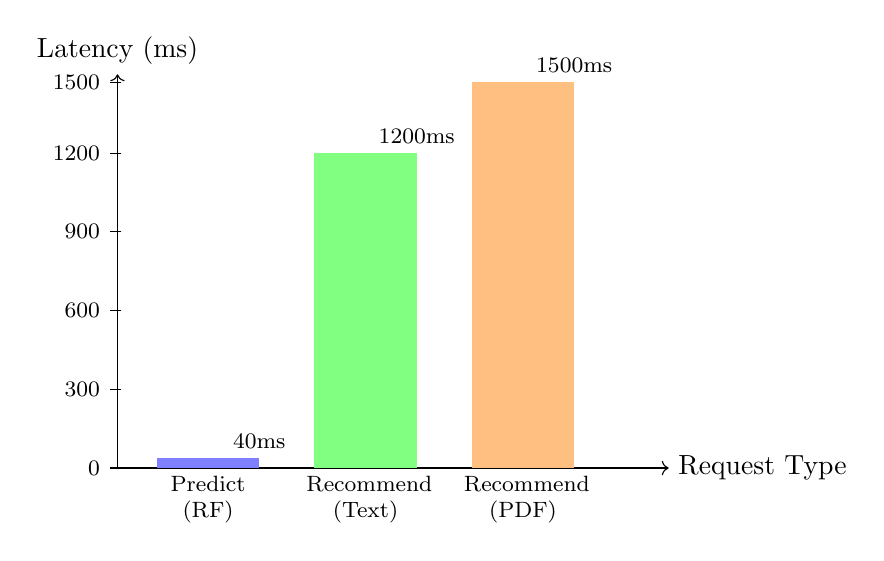
\begin{tikzpicture}
  \begin{scope}
    % Axes
    \draw[->] (0,0) -- (7,0) node[right] {Request Type};
    \draw[->] (0,0) -- (0,5) node[above] {Latency (ms)};

    % Y-axis labels
    \foreach \y/\label in {0/0, 1/300, 2/600, 3/900, 4/1200, 4.9/1500}
      \draw (0.05,\y) -- (-0.1,\y) node[left, font=\footnotesize] {\label};

    % Bars
    \fill[blue!50] (0.5,0) rectangle (1.8, 0.13) node[above, font=\footnotesize, black] {40ms};
    \fill[green!50] (2.5,0) rectangle (3.8, 4.0) node[above, font=\footnotesize, black] {1200ms};
    \fill[orange!50] (4.5,0) rectangle (5.8, 4.9) node[above, font=\footnotesize, black] {1500ms};

    % X-axis labels
    \node[font=\footnotesize, text width=1.5cm, align=center] at (1.15, -0.4) {Predict\\ (RF)};
    \node[font=\footnotesize, text width=1.5cm, align=center] at (3.15, -0.4) {Recommend\\ (Text)};
    \node[font=\footnotesize, text width=1.5cm, align=center] at (5.15, -0.4) {Recommend\\ (PDF)};
  \end{scope}
\end{tikzpicture}
\caption{API response latency comparison across endpoint types}
\label{fig:latency_bar}
\end{figure}

\section{Discussion}

\subsection{Dual-AI Complementarity}
The system's dual-AI approach proves highly effective. The local Random Forest model provides near-instantaneous, privacy-preserving disease classification from structured symptom inputs. The Groq LLM complements this by handling unstructured free-text inputs and semi-structured PDF clinical documents---a task the classical ML model is architecturally incapable of performing. Together, they cover a broad spectrum of real-world patient input modalities.

\subsection{API Deprecation Handling}
A significant practical challenge encountered during development was the upstream deprecation of Groq's \texttt{llama-3.2-11b-vision-preview} model. This model had been planned for processing raw image uploads (JPG/PNG). Its decommissioning required a rapid architectural pivot: the system was refactored to explicitly reject image uploads with a descriptive, user-friendly error message and to instead favor PDF text extraction via \texttt{PyPDF2}. This demonstrates the importance of building graceful degradation logic into AI-dependent systems, as external API surfaces are subject to change without warning.

\subsection{User Experience Refinements}
User testing feedback drove two significant UI improvements:
\begin{itemize}
    \item \textbf{Cancel Upload Button:} The initial file input provided no mechanism to deselect an uploaded file. A ``Remove'' button was added that clears the React state variable, replacing the file pill with the original file input field.
    \item \textbf{Two-Column Card Layout:} The original single-column form layout placed the file upload section far below the fold, making it easy to miss. Refactoring to a side-by-side two-card CSS Grid layout made both input options immediately visible and equally prominent.
\end{itemize}

\subsection{Limitations Observed in Practice}
\begin{itemize}
    \item \textbf{Scanned PDFs:} Patients who save screenshots of their reports as PDF files produce documents where all content is embedded as image data. \texttt{PyPDF2} cannot extract text from such files. The system correctly handles this by returning a descriptive error, but a future enhancement would involve integrating an OCR library (such as \texttt{pytesseract}) for scanned document support.
    \item \textbf{Groq Rate Limiting:} Under high usage, the Groq API may return HTTP 429 (Too Many Requests). The frontend implements a countdown timer to transparently inform the user of the retry window.
    \item \textbf{RF Model Coverage:} The Random Forest model is limited to the 41 disease classes and 132 symptoms defined in its training dataset. Rare or novel diseases outside this scope cannot be predicted.
\end{itemize}

\chapter{CONCLUSION AND FUTURE WORK}

\section{Conclusion}

MedPredictX successfully demonstrates the feasibility and practical utility of integrating classical machine learning and modern Large Language Models into a single, cohesive, production-grade healthcare triage web application. The system directly addresses the well-documented shortcomings of existing first-generation telemedicine platforms by introducing two intelligent AI engines that complement each other across different patient input modalities.

The \textbf{Local Random Forest Classifier}, trained on 4,920 patient symptom records across 41 disease classes, achieves a test accuracy of 97.87\% while delivering sub-40ms inference latency. This exceeds the 200ms response time requirement defined in the SRS, providing a near-instantaneous user experience. The model operates entirely on local hardware, guaranteeing patient data privacy and ensuring that the prediction service remains available even in the absence of internet connectivity.

The \textbf{Groq LLM-powered AI Recommender} extends the system's capabilities far beyond what a classical classifier can achieve, accepting free-form natural language symptom descriptions and machine-extracted text from PDF medical reports. It outputs a highly structured, actionable recommendation---including the appropriate medical specialty, urgency assessment, key reasoning, self-care tips, and a dynamically generated Google Maps specialist geo-location link. This bridges the critical last-mile gap between digital triage and physical clinical care.

The \textbf{Unified Medical Triage Hub} consolidates both tools into a single, professionally designed React page with a smooth tabbed interface, eliminating navigational friction and presenting a cohesive user experience. The two-column card layout within the AI Recommender unambiguously presents both input options to the user, improving discoverability and reducing task completion friction.

From a software engineering perspective, this project demonstrates the critical importance of designing for API instability: the graceful deprecation handling of the Groq Vision model, the replacement of image-analysis with PDF text extraction, and the clear user communication via descriptive error messages all exemplify production-grade resilience engineering principles.

\section{Future Work}

While the current iteration of MedPredictX is fully functional and clinically relevant as an informational triage tool, several high-value enhancements are identified for future development iterations:

\begin{enumerate}
    \item \textbf{OCR for Scanned PDFs:} Integrating an OCR library such as \texttt{pytesseract} (backed by the Tesseract engine) would enable the AI Recommender to analyze scanned or photographed medical documents, removing the current limitation that only digital-native PDFs with embedded text are supported.

    \item \textbf{EHR/FHIR Integration:} Implementing HL7 FHIR (Fast Healthcare Interoperability Resources) API connectors would allow MedPredictX to directly import patient medical histories from compliant Electronic Health Record systems, dramatically enriching the context available to the LLM recommender.

    \item \textbf{Real-Time Video Consultation:} Integrating WebRTC-based peer-to-peer video channels would enable seamless handoff from the AI triage to a live telemedicine consultation with a platform-registered Doctor, creating a complete end-to-end clinical encounter within a single platform.

    \item \textbf{Voice Input:} Integrating the Web Speech API or the Groq Whisper model (for high-accuracy speech-to-text) would allow patients to verbally describe their symptoms, making the platform significantly more accessible to elderly users or those with limited typing ability.

    \item \textbf{IoT Vital Signs Integration:} A REST endpoint could be exposed to accept real-time vital sign data (heart rate, blood pressure, SpO2) from consumer-grade IoT wearables. This data could be included in the LLM prompt context to substantially increase the accuracy and relevance of triage recommendations.

    \item \textbf{Fine-tuned Medical LLM:} The current implementation uses a general-purpose LLM with a carefully engineered system prompt. Fine-tuning a smaller, dedicated model (such as Llama 3.1 8B) on a curated medical QA dataset would improve recommendation consistency and reduce the risk of hallucination in clinical contexts.

    \item \textbf{Production Deployment:} Migrating from SQLite to PostgreSQL, deploying on a cloud platform (e.g., AWS EC2 or DigitalOcean), configuring NGINX as a reverse proxy, and enabling HTTPS via Let's Encrypt certificates would constitute a production-ready deployment.
\end{enumerate}

\chapter{REFERENCES}
\addcontentsline{toc}{chapter}{References}

\begin{thebibliography}{99}

\bibitem{breiman2001}
L. Breiman, ``Random Forests,'' \textit{Machine Learning}, vol. 45, no. 1, pp. 5--32, Oct. 2001.

\bibitem{vaswani2017}
A. Vaswani, N. Shazeer, N. Parmar, J. Uszkoreit, L. Jones, A. N. Gomez, L. Kaiser, and I. Polosukhin, ``Attention Is All You Need,'' in \textit{Advances in Neural Information Processing Systems (NeurIPS)}, vol. 30, 2017.

\bibitem{lee2020}
J. Lee, W. Yoon, S. Kim, D. Kim, S. Kim, C. H. So, and J. Kang, ``BioBERT: A Pre-trained Biomedical Language Representation Model for Biomedical Text Mining,'' \textit{Bioinformatics}, vol. 36, no. 4, pp. 1234--1240, Feb. 2020.

\bibitem{alsentzer2019}
E. Alsentzer, J. R. Murphy, W. Boag, W. Weng, D. Jin, T. Naumann, and M. McDermott, ``Publicly Available Clinical BERT Embeddings,'' in \textit{Proceedings of the 2nd Clinical NLP Workshop}, Minneapolis, MN, 2019.

\bibitem{django2024}
Django Software Foundation, ``Django Documentation, Version 4.2,'' \url{https://docs.djangoproject.com/}, 2024.

\bibitem{react2024}
Meta Open Source, ``React: A JavaScript Library for Building User Interfaces,'' \url{https://reactjs.org/}, 2024.

\bibitem{sklearn2011}
F. Pedregosa, G. Varoquaux, A. Gramfort, V. Michel, B. Thirion, O. Grisel, M. Blondel, P. Prettenhofer, R. Weiss, V. Dubourg, J. Vanderplas, A. Passos, D. Cournapeau, M. Brucher, M. Perrot, and E. Duchesnay, ``Scikit-learn: Machine Learning in Python,'' \textit{Journal of Machine Learning Research}, vol. 12, pp. 2825--2830, 2011.

\bibitem{groq2024}
Groq Inc., ``Groq API Documentation --- Fast AI Inference,'' \url{https://console.groq.com/docs}, 2024.

\bibitem{ieee830}
IEEE, ``IEEE Recommended Practice for Software Requirements Specifications,'' \textit{IEEE Std 830-1998}, 1998.

\bibitem{jwt2015}
M. Jones, J. Bradley, and N. Sakimura, ``JSON Web Token (JWT),'' \textit{RFC 7519}, Internet Engineering Task Force (IETF), May 2015.

\bibitem{pypdf2}
M. Fenniak and contributors, ``PyPDF2: A Python library for PDF file manipulation,'' \url{https://pypdf2.readthedocs.io/}, 2024.

\bibitem{vite2024}
Evan You and contributors, ``Vite: Next Generation Frontend Tooling,'' \url{https://vitejs.dev/}, 2024.

\bibitem{framermotion2024}
Framer Ltd., ``Framer Motion: A production-ready motion library for React,'' \url{https://www.framer.com/motion/}, 2024.

\bibitem{joblib2024}
Joblib Development Team, ``Joblib: Running Python Functions as Pipeline Jobs,'' \url{https://joblib.readthedocs.io/}, 2024.

\end{thebibliography}


\appendix
\chapter{Appendix A: System Architecture Diagrams}
\addcontentsline{toc}{chapter}{Appendix A: System Architecture Diagrams}

\section{Box-and-Line Architecture Diagram}

Figure~\ref{fig:boxline} provides a high-level box-and-line representation of the complete MedPredictX system, showing the major components and their communication channels.

\begin{figure}[htbp]
\centering
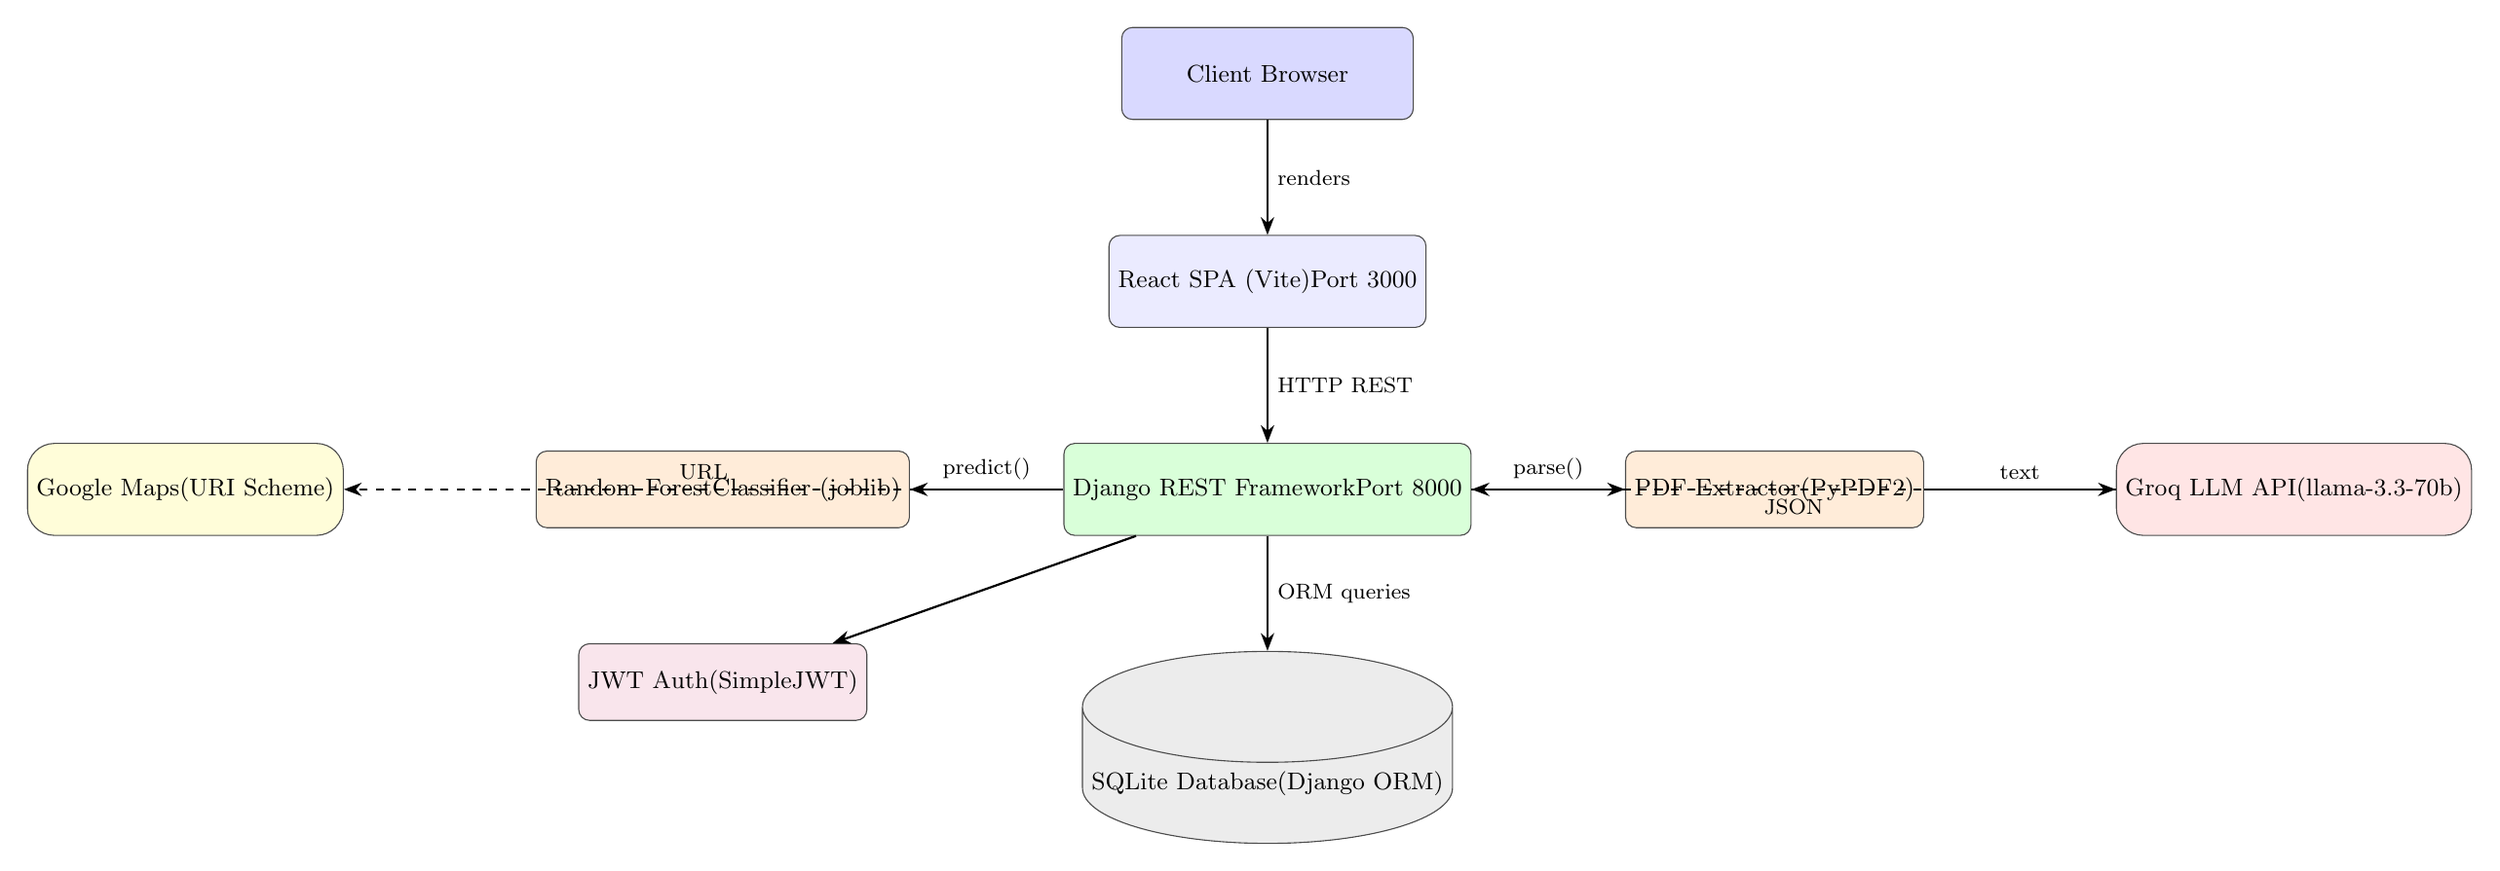
\begin{tikzpicture}[node distance=1.5cm and 2.5cm, every node/.style={font=\small}]
  % Client
  \node[block, fill=blue!15, minimum width=3.8cm, minimum height=1.2cm] (client) {Client Browser};

  % Frontend box
  \node[block, fill=blue!8, minimum width=3.8cm, minimum height=1.2cm, below=1.5cm of client] (spa) {React SPA (Vite)\\Port 3000};

  % Backend box
  \node[block, fill=green!15, minimum width=3.8cm, minimum height=1.2cm, below=1.5cm of spa] (backend) {Django REST Framework\\Port 8000};

  % Internal services
  \node[block, fill=orange!15, minimum width=3cm, minimum height=1cm, left=2cm of backend] (rf) {Random Forest\\Classifier (joblib)};
  \node[block, fill=orange!15, minimum width=3cm, minimum height=1cm, right=2cm of backend] (pdf) {PDF Extractor\\(PyPDF2)};

  % Database
  \node[db, fill=gray!15, minimum width=3cm, minimum height=1cm, below=1.5cm of backend] (db) {SQLite Database\\(Django ORM)};

  % External
  \node[cloud, fill=red!10, minimum width=3.5cm, minimum height=1.2cm, right=2.5cm of pdf] (groq) {Groq LLM API\\(llama-3.3-70b)};
  \node[cloud, fill=yellow!15, minimum width=3.5cm, minimum height=1.2cm, left=2.5cm of rf] (maps) {Google Maps\\(URI Scheme)};

  % Auth
  \node[block, fill=purple!10, minimum width=3cm, minimum height=1cm, below=1.5cm of rf] (jwt) {JWT Auth\\(SimpleJWT)};

  % Connections
  \draw[arrow] (client) -- node[right, font=\footnotesize]{renders} (spa);
  \draw[arrow] (spa) -- node[right, font=\footnotesize]{HTTP REST} (backend);
  \draw[arrow] (backend) -- node[above, font=\footnotesize]{predict()} (rf);
  \draw[arrow] (backend) -- node[above, font=\footnotesize]{parse()} (pdf);
  \draw[arrow] (backend) -- node[right, font=\footnotesize]{ORM queries} (db);
  \draw[arrow] (pdf) -- node[above, font=\footnotesize]{text} (groq);
  \draw[dasharrow] (groq) -- node[below, font=\footnotesize]{JSON} (backend);
  \draw[dasharrow] (backend) -- node[above, font=\footnotesize]{URL} (maps);
  \draw[arrow] (backend) -- (jwt);
\end{tikzpicture}
\caption{Complete box-and-line system architecture diagram for MedPredictX}
\label{fig:boxline}
\end{figure}

\section{Data Flow Diagram (Level 0 --- Context Diagram)}

Figure~\ref{fig:dfd0} shows the Level 0 Data Flow Diagram (Context Diagram) for the MedPredictX system.

\begin{figure}[htbp]
\centering
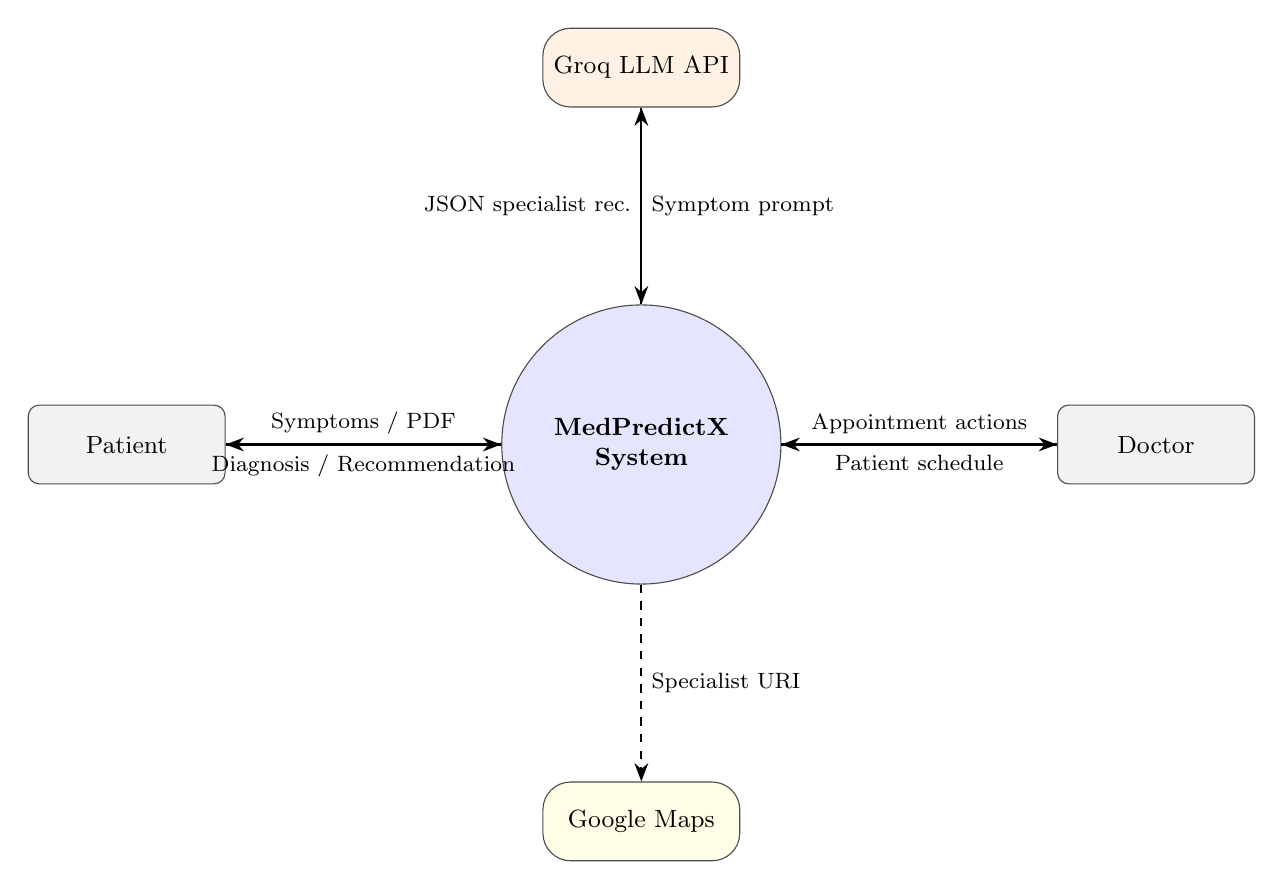
\begin{tikzpicture}[node distance=3.5cm, every node/.style={font=\small}]
  % Central process
  \node[circle, draw=black!70, fill=blue!10, minimum width=3.5cm, text centered, text width=3.2cm] (sys) {\textbf{MedPredictX\\System}};

  % External entities
  \node[block, fill=gray!10, left=3.5cm of sys, minimum width=2.5cm] (patient) {Patient};
  \node[block, fill=gray!10, right=3.5cm of sys, minimum width=2.5cm] (doctor) {Doctor};
  \node[cloud, fill=orange!10, above=2.5cm of sys, minimum width=2.5cm] (groq2) {Groq LLM API};
  \node[cloud, fill=yellow!10, below=2.5cm of sys, minimum width=2.5cm] (maps2) {Google Maps};

  % Flows
  \draw[arrow] (patient) -- node[above, font=\footnotesize]{Symptoms / PDF} (sys);
  \draw[arrow] (sys) -- node[below, font=\footnotesize]{Diagnosis / Recommendation} (patient);
  \draw[arrow] (doctor) -- node[above, font=\footnotesize]{Appointment actions} (sys);
  \draw[arrow] (sys) -- node[below, font=\footnotesize]{Patient schedule} (doctor);
  \draw[arrow] (sys) -- node[right, font=\footnotesize]{Symptom prompt} (groq2);
  \draw[arrow] (groq2) -- node[left, font=\footnotesize]{JSON specialist rec.} (sys);
  \draw[dasharrow] (sys) -- node[right, font=\footnotesize]{Specialist URI} (maps2);
\end{tikzpicture}
\caption{Level 0 Context Data Flow Diagram for MedPredictX}
\label{fig:dfd0}
\end{figure}

\section{Data Flow Diagram (Level 1)}

Figure~\ref{fig:dfd1} decomposes the system into its major internal processes.

\begin{figure}[htbp]
\centering
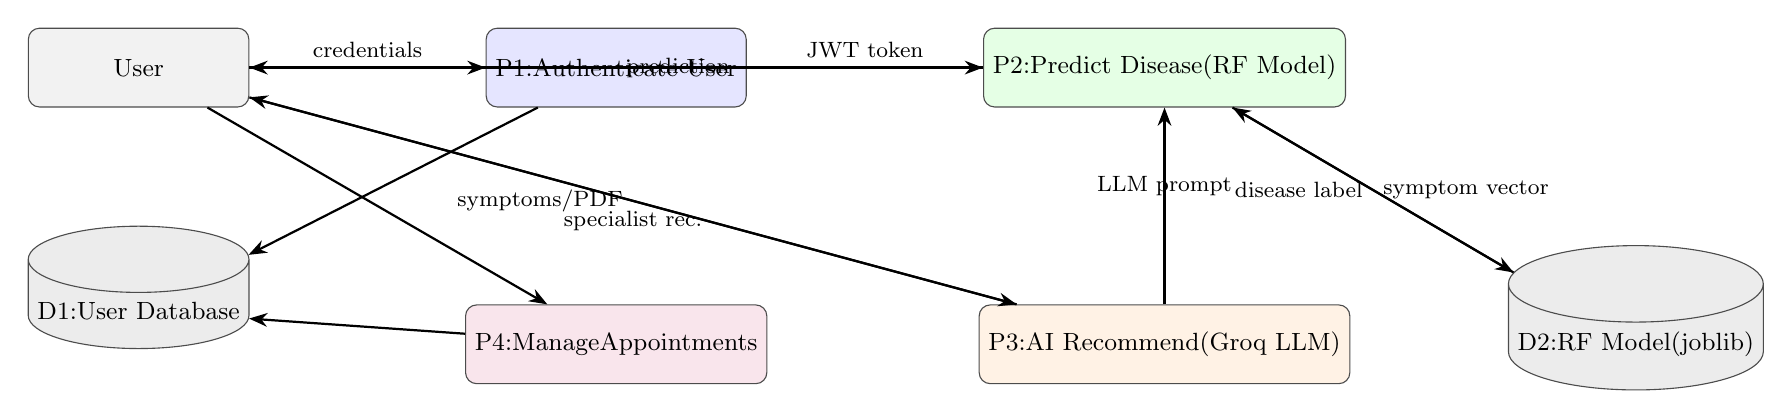
\begin{tikzpicture}[node distance=2.5cm and 3.5cm, every node/.style={font=\footnotesize}]
  % External entity
  \node[block, fill=gray!10] (user) {User};

  % Processes
  \node[block, fill=blue!10, right=3cm of user] (auth) {P1:\\Authenticate User};
  \node[block, fill=green!10, right=3cm of auth] (predict) {P2:\\Predict Disease\\(RF Model)};
  \node[block, fill=orange!10, below=2.5cm of predict] (recommend) {P3:\\AI Recommend\\(Groq LLM)};
  \node[block, fill=purple!10, below=2.5cm of auth] (appt) {P4:\\Manage\\Appointments};

  % Data stores
  \node[db, fill=gray!15, below=1.5cm of user, minimum width=2.5cm] (userdb) {D1:\\User Database};
  \node[db, fill=gray!15, right=2cm of recommend, minimum width=2.5cm] (modeldb) {D2:\\RF Model\\(joblib)};

  % Flows
  \draw[arrow] (user) -- node[above]{credentials} (auth);
  \draw[arrow] (auth) -- node[above]{JWT token} (predict);
  \draw[arrow] (auth) -- (userdb);
  \draw[arrow] (predict) -- node[right]{symptom vector} (modeldb);
  \draw[arrow] (modeldb) -- node[left]{disease label} (predict);
  \draw[arrow] (predict) -- node[right]{prediction} (user);
  \draw[arrow] (recommend) -- node[above]{LLM prompt} (predict);
  \draw[arrow] (user) -- node[left]{symptoms/PDF} (recommend);
  \draw[arrow] (recommend) -- node[below]{specialist rec.} (user);
  \draw[arrow] (user) -- (appt);
  \draw[arrow] (appt) -- (userdb);
\end{tikzpicture}
\caption{Level 1 Data Flow Diagram showing internal MedPredictX processes}
\label{fig:dfd1}
\end{figure}

\chapter{Appendix B: UML Design Models}
\addcontentsline{toc}{chapter}{Appendix B: UML Design Models}

\section{Use Case Diagram}

Figure~\ref{fig:usecase} shows the primary use cases for each actor in the MedPredictX system.

\begin{figure}[htbp]
\centering
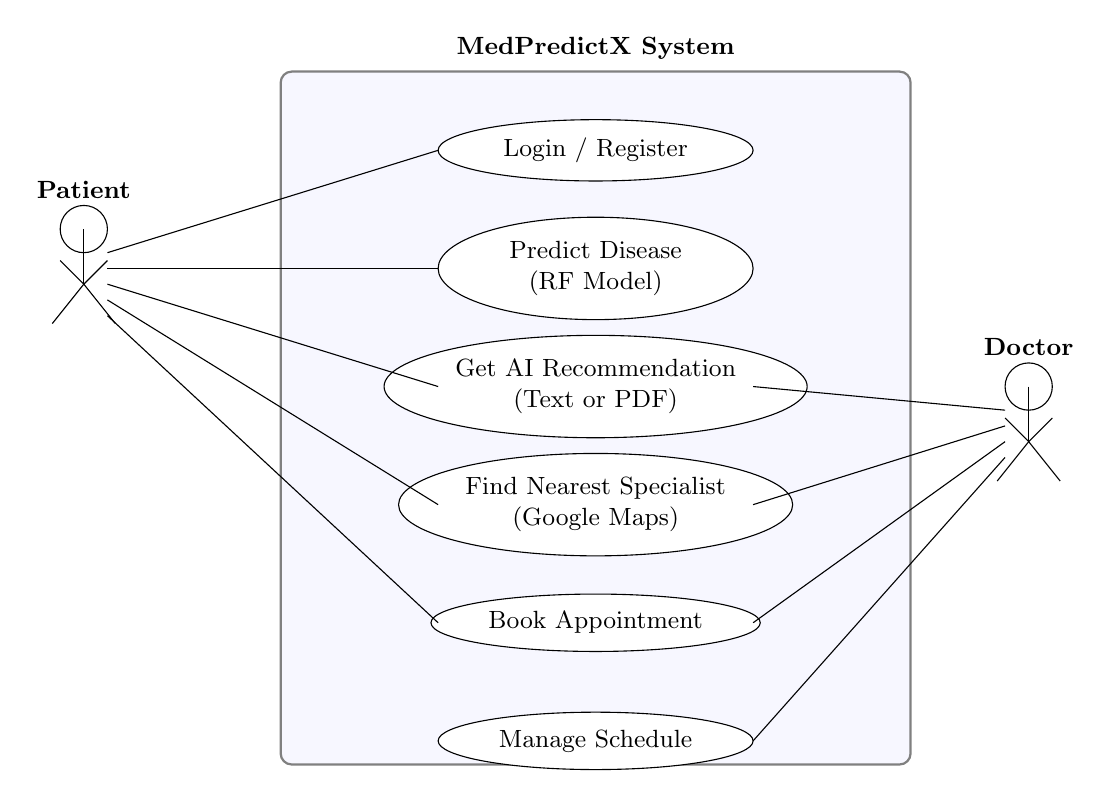
\begin{tikzpicture}[every node/.style={font=\small}]
  % System boundary
  \draw[rounded corners, draw=black!50, fill=blue!3, thick] (1.5,-0.3) rectangle (9.5,8.5);
  \node at (5.5, 8.8) {\textbf{MedPredictX System}};

  % Patient actor
  \node[font=\small] at (-1, 7) {\textbf{Patient}};
  \draw (-1,6.5) circle (0.3);
  \draw (-1,6.5) -- (-1,5.8);
  \draw (-1,5.8) -- (-1.4,5.3);
  \draw (-1,5.8) -- (-0.6,5.3);
  \draw (-1,5.8) -- (-1.3,6.1);
  \draw (-1,5.8) -- (-0.7,6.1);

  % Doctor actor
  \node[font=\small] at (11, 5) {\textbf{Doctor}};
  \draw (11,4.5) circle (0.3);
  \draw (11,4.5) -- (11,3.8);
  \draw (11,3.8) -- (11.4,3.3);
  \draw (11,3.8) -- (10.6,3.3);
  \draw (11,3.8) -- (11.3,4.1);
  \draw (11,3.8) -- (10.7,4.1);

  % Use cases
  \node[ellipse, draw, fill=white, minimum width=4cm, align=center] (login) at (5.5,7.5) {Login / Register};
  \node[ellipse, draw, fill=white, minimum width=4cm, align=center] (predict) at (5.5,6) {Predict Disease\\(RF Model)};
  \node[ellipse, draw, fill=white, minimum width=4cm, align=center] (recommend) at (5.5,4.5) {Get AI Recommendation\\(Text or PDF)};
  \node[ellipse, draw, fill=white, minimum width=4cm, align=center] (maps) at (5.5,3) {Find Nearest Specialist\\(Google Maps)};
  \node[ellipse, draw, fill=white, minimum width=4cm, align=center] (appt) at (5.5,1.5) {Book Appointment};
  \node[ellipse, draw, fill=white, minimum width=4cm, align=center] (schedule) at (5.5,0) {Manage Schedule};

  % Patient connections
  \draw (-0.7,6.2) -- (3.5,7.5);
  \draw (-0.7,6.0) -- (3.5,6);
  \draw (-0.7,5.8) -- (3.5,4.5);
  \draw (-0.7,5.6) -- (3.5,3);
  \draw (-0.7,5.4) -- (3.5,1.5);

  % Doctor connections
  \draw (10.7,4.2) -- (7.5,4.5);
  \draw (10.7,4.0) -- (7.5,3);
  \draw (10.7,3.8) -- (7.5,1.5);
  \draw (10.7,3.6) -- (7.5,0);
\end{tikzpicture}
\caption{Use case diagram showing actor interactions with MedPredictX}
\label{fig:usecase}
\end{figure}

\section{Activity Diagram: Disease Prediction Flow}

Figure~\ref{fig:activity_predict} shows the complete activity flow for the Local Disease Prediction feature.

\begin{figure}[htbp]
\centering
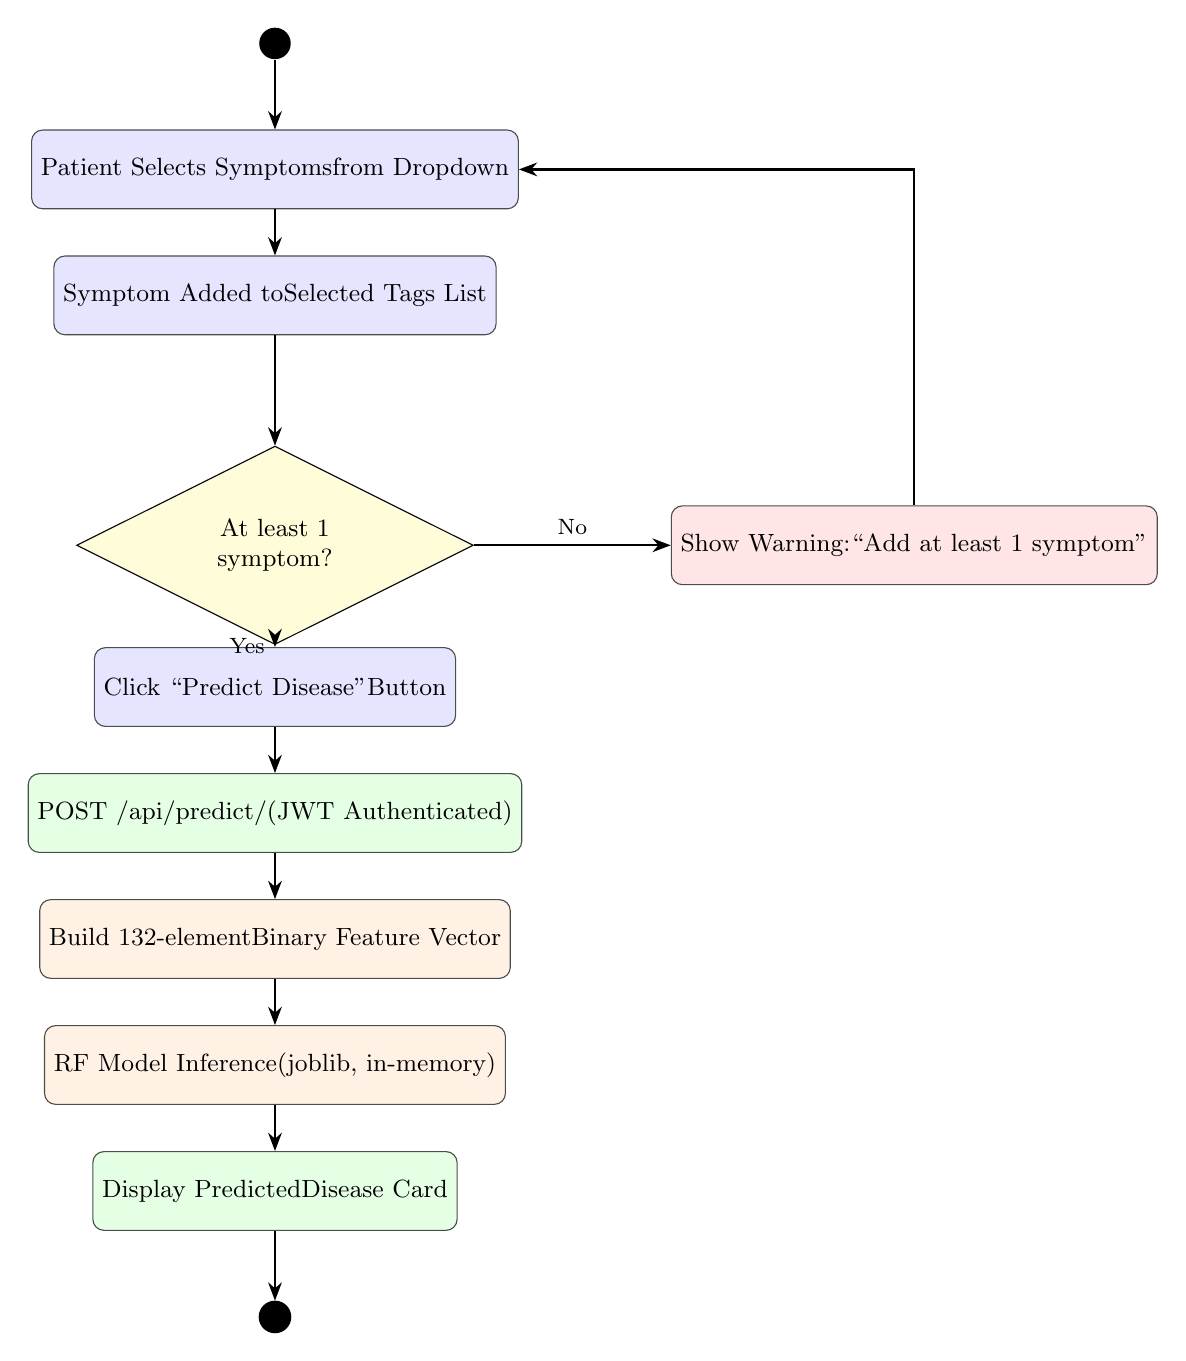
\begin{tikzpicture}[node distance=1.6cm, every node/.style={font=\small}]
  % Start
  \node[circle, fill=black, minimum size=0.4cm] (start) {};
  \node[block, fill=blue!10, below of=start] (select) {Patient Selects Symptoms\\from Dropdown};
  \node[block, fill=blue!10, below of=select] (add) {Symptom Added to\\Selected Tags List};
  \node[diamond, aspect=2, draw, fill=yellow!15, below=1.4cm of add, text width=3cm, align=center] (enough) {At least 1\\symptom?};
  \node[block, fill=blue!10, below of=enough, node distance=1.8cm] (submit) {Click ``Predict Disease''\\Button};
  \node[block, fill=green!10, below of=submit] (api) {POST /api/predict/\\(JWT Authenticated)};
  \node[block, fill=orange!10, below of=api] (vector) {Build 132-element\\Binary Feature Vector};
  \node[block, fill=orange!10, below of=vector] (model) {RF Model Inference\\(joblib, in-memory)};
  \node[block, fill=green!10, below of=model] (display) {Display Predicted\\Disease Card};
  \node[circle, draw, fill=black, minimum size=0.4cm, below of=display] (end) {};
  \node[block, fill=red!10, right=2.5cm of enough] (warn) {Show Warning:\\``Add at least 1 symptom''};

  \draw[arrow] (start) -- (select);
  \draw[arrow] (select) -- (add);
  \draw[arrow] (add) -- (enough);
  \draw[arrow] (enough) -- node[left, font=\footnotesize]{Yes} (submit);
  \draw[arrow] (enough) -- node[above, font=\footnotesize]{No} (warn);
  \draw[arrow] (warn) |- (select);
  \draw[arrow] (submit) -- (api);
  \draw[arrow] (api) -- (vector);
  \draw[arrow] (vector) -- (model);
  \draw[arrow] (model) -- (display);
  \draw[arrow] (display) -- (end);
\end{tikzpicture}
\caption{Activity diagram for Local Disease Prediction workflow}
\label{fig:activity_predict}
\end{figure}

\section{Activity Diagram: AI Recommendation Flow}

Figure~\ref{fig:activity_recommend} shows the activity flow for the AI Specialist Recommender feature.

\begin{figure}[htbp]
\centering
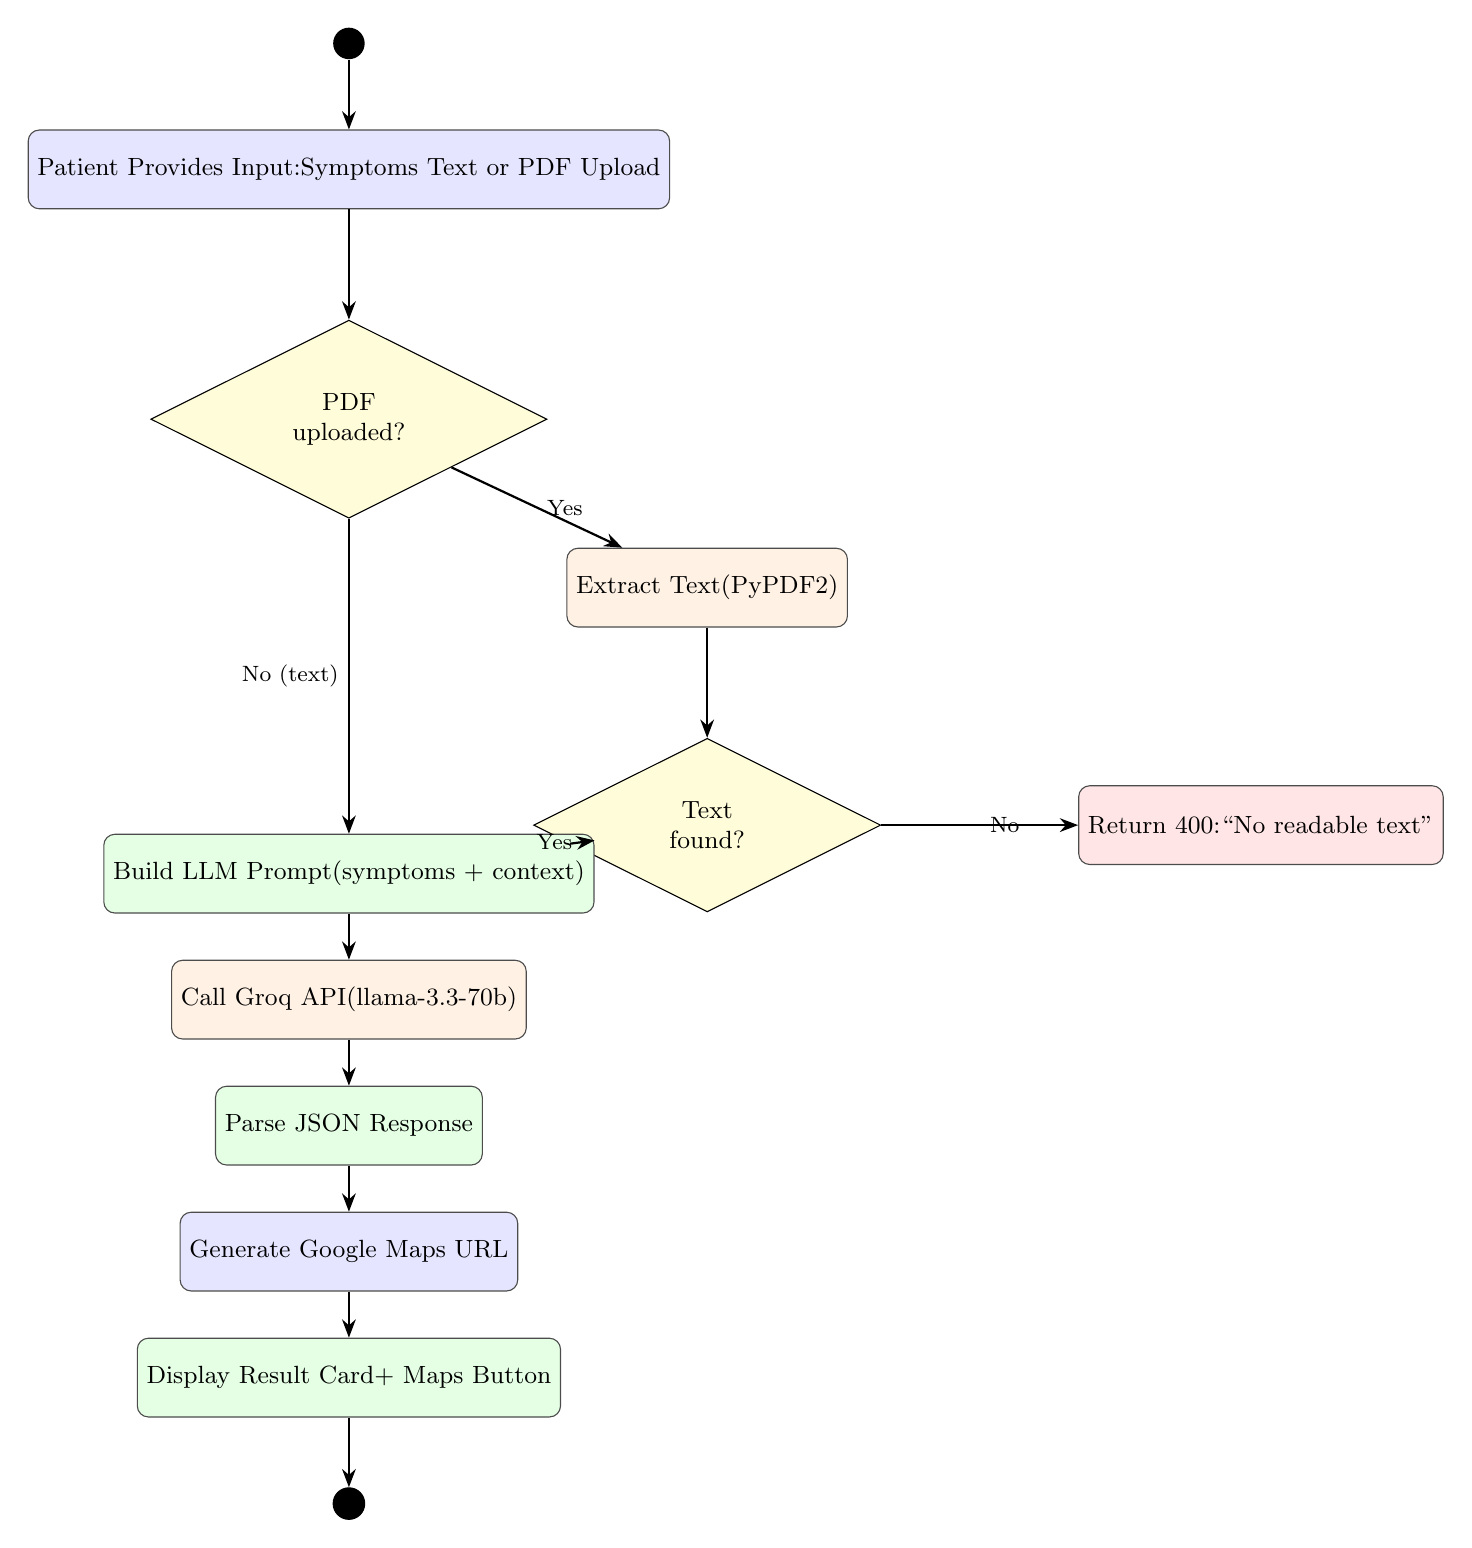
\begin{tikzpicture}[node distance=1.6cm, every node/.style={font=\small}]
  \node[circle, fill=black, minimum size=0.4cm] (start) {};
  \node[block, fill=blue!10, below of=start] (input) {Patient Provides Input:\\Symptoms Text or PDF Upload};
  \node[diamond, aspect=2, draw, fill=yellow!15, below=1.4cm of input, text width=3cm, align=center] (hasfile) {PDF\\uploaded?};
  \node[block, fill=orange!10, below right=1cm and 1.5cm of hasfile] (extract) {Extract Text\\(PyPDF2)};
  \node[diamond, aspect=2, draw, fill=yellow!15, below=1.4cm of extract, text width=2.5cm, align=center] (hastext) {Text\\found?};
  \node[block, fill=red!10, right=2.5cm of hastext] (err) {Return 400:\\``No readable text''};
  \node[block, fill=green!10, below=4cm of hasfile] (prompt) {Build LLM Prompt\\(symptoms + context)};
  \node[block, fill=orange!10, below of=prompt] (groq3) {Call Groq API\\(llama-3.3-70b)};
  \node[block, fill=green!10, below of=groq3] (parse) {Parse JSON Response};
  \node[block, fill=blue!10, below of=parse] (mapurl) {Generate Google Maps URL};
  \node[block, fill=green!10, below of=mapurl] (show) {Display Result Card\\+ Maps Button};
  \node[circle, draw, fill=black, minimum size=0.4cm, below of=show] (end) {};

  \draw[arrow] (start) -- (input);
  \draw[arrow] (input) -- (hasfile);
  \draw[arrow] (hasfile) -- node[right, font=\footnotesize]{Yes} (extract);
  \draw[arrow] (hasfile) -- node[left, font=\footnotesize]{No (text)} (prompt);
  \draw[arrow] (extract) -- (hastext);
  \draw[arrow] (hastext) -- node[right, font=\footnotesize]{No} (err);
  \draw[arrow] (hastext) -- node[left, font=\footnotesize]{Yes} (prompt);
  \draw[arrow] (prompt) -- (groq3);
  \draw[arrow] (groq3) -- (parse);
  \draw[arrow] (parse) -- (mapurl);
  \draw[arrow] (mapurl) -- (show);
  \draw[arrow] (show) -- (end);
\end{tikzpicture}
\caption{Activity diagram for AI Specialist Recommendation workflow}
\label{fig:activity_recommend}
\end{figure}

\section{State Machine Diagram: Triage Hub}

Figure~\ref{fig:state} shows the state machine for the Unified Medical Triage Hub UI component.

\begin{figure}[htbp]
\centering
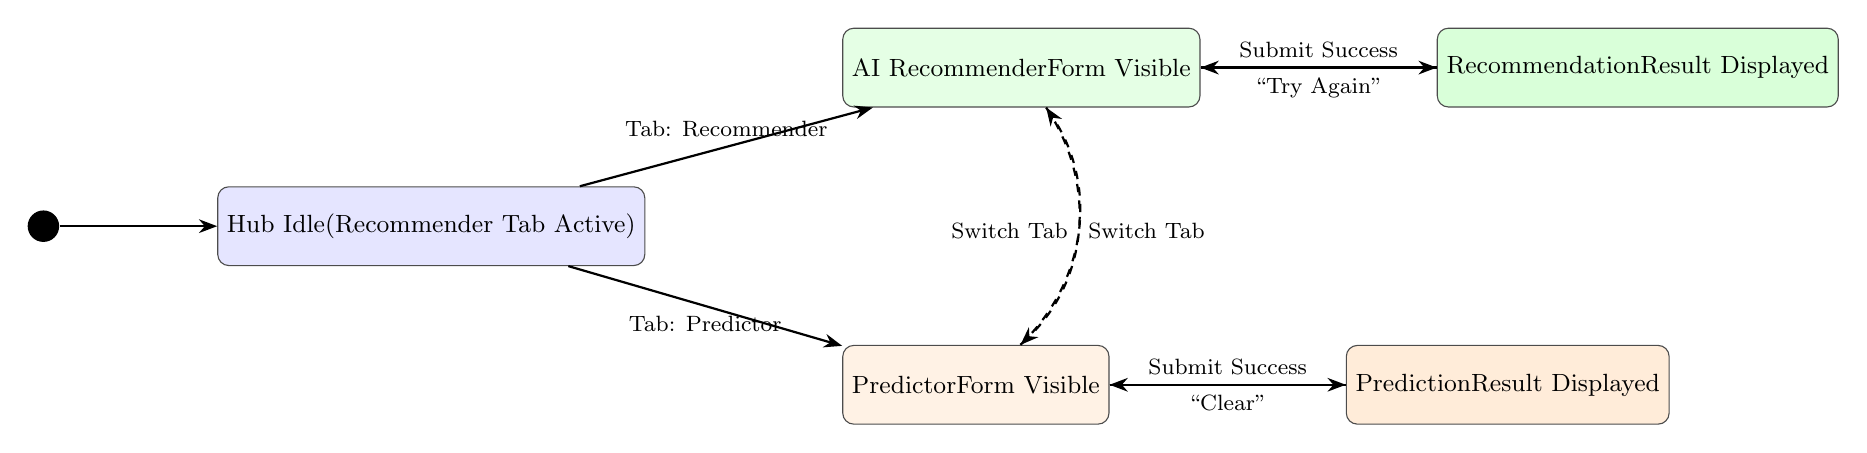
\begin{tikzpicture}[node distance=2.5cm and 3cm, every node/.style={font=\small}]
  \node[circle, fill=black, minimum size=0.4cm] (initial) {};
  \node[block, fill=blue!10, right=2cm of initial] (hub) {Hub Idle\\(Recommender Tab Active)};
  \node[block, fill=green!10, above right=1cm and 2.5cm of hub] (recommender) {AI Recommender\\Form Visible};
  \node[block, fill=orange!10, below right=1cm and 2.5cm of hub] (predictor) {Predictor\\Form Visible};
  \node[block, fill=green!15, right=3cm of recommender] (recresult) {Recommendation\\Result Displayed};
  \node[block, fill=orange!15, right=3cm of predictor] (predresult) {Prediction\\Result Displayed};

  \draw[arrow] (initial) -- (hub);
  \draw[arrow] (hub) -- node[above, font=\footnotesize]{Tab: Recommender} (recommender);
  \draw[arrow] (hub) -- node[below, font=\footnotesize]{Tab: Predictor} (predictor);
  \draw[arrow] (recommender) -- node[above, font=\footnotesize]{Submit Success} (recresult);
  \draw[arrow] (recresult) -- node[below, font=\footnotesize]{``Try Again''} (recommender);
  \draw[arrow] (predictor) -- node[above, font=\footnotesize]{Submit Success} (predresult);
  \draw[arrow] (predresult) -- node[below, font=\footnotesize]{``Clear''} (predictor);
  \draw[dasharrow, bend left=40] (recommender) to node[left, font=\footnotesize]{Switch Tab} (predictor);
  \draw[dasharrow, bend right=40] (predictor) to node[right, font=\footnotesize]{Switch Tab} (recommender);
\end{tikzpicture}
\caption{State machine diagram for the Unified Medical Triage Hub component}
\label{fig:state}
\end{figure}


\end{document}
